\documentclass[12pt]{article}

\usepackage{fullpage}
\usepackage{graphicx, rotating, booktabs} 
\usepackage{times}
\usepackage{fbb} 
\usepackage{natbib} 
\usepackage{indentfirst} 
\usepackage{setspace}
\usepackage{grffile} 
\usepackage{hyperref}
\usepackage{adjustbox}
\usepackage{multirow} 
\usepackage{amsmath}
\usepackage[labelfont={bf},textfont=it,labelsep=period]{caption}
\setcitestyle{aysep{}}
\usepackage{sectsty}
% for the big table
\usepackage{afterpage}
\usepackage{array}
\usepackage{lscape}
\usepackage{longtable}
\usepackage{float}
\sectionfont{\Large}
\subsectionfont{\noindent\large\textit}
\subsubsectionfont{\normalsize}


\singlespace
\title{\textbf{Appendix: Arms and Electoral Influence: How Arms Deals with Autocracies Shape Defense Contracting in the United States}}
%\author{Joshua Alley} 
\date{}

\bibliographystyle{apsr}

\begin{document}

\maketitle 

\singlespace 

\tableofcontents

\bigskip





\section{Arms Deals Count Model Check}

In this section, I check the results of hurdle Poisson models of US arms deals in three steps. 
First, I show similar patterns in raw data. 
Second, I demonstrate that OLS, Poisson, and zero-inflated Poisson models give similar inferences to the hurdle Poisson models in the manuscript. 
Finally, I use posterior predictive checks for the hurdle Poisson model and a negative binomial model to show that a Poisson outcome likelihood fits the observed data better. 


\subsection{Raw Data}

The pattern of increasing arms deals with autocratic allies as presidential elections approach is evident in raw data.
\autoref{fig:deals-democ-raw} plot the number of arms deals per country after dividing state-year observations based on years to a presidential election, four quartiles of democracy, and whether a country is an ally of the United States.
Autocratic U.S. allies average more than one additional deal in election years than in years immediately after an election. 
More democratic allies receive more arms deals than non-allied states, but deals with these countries do not track the electoral cycle. 


\begin{figure}[htpb]
	\centering
		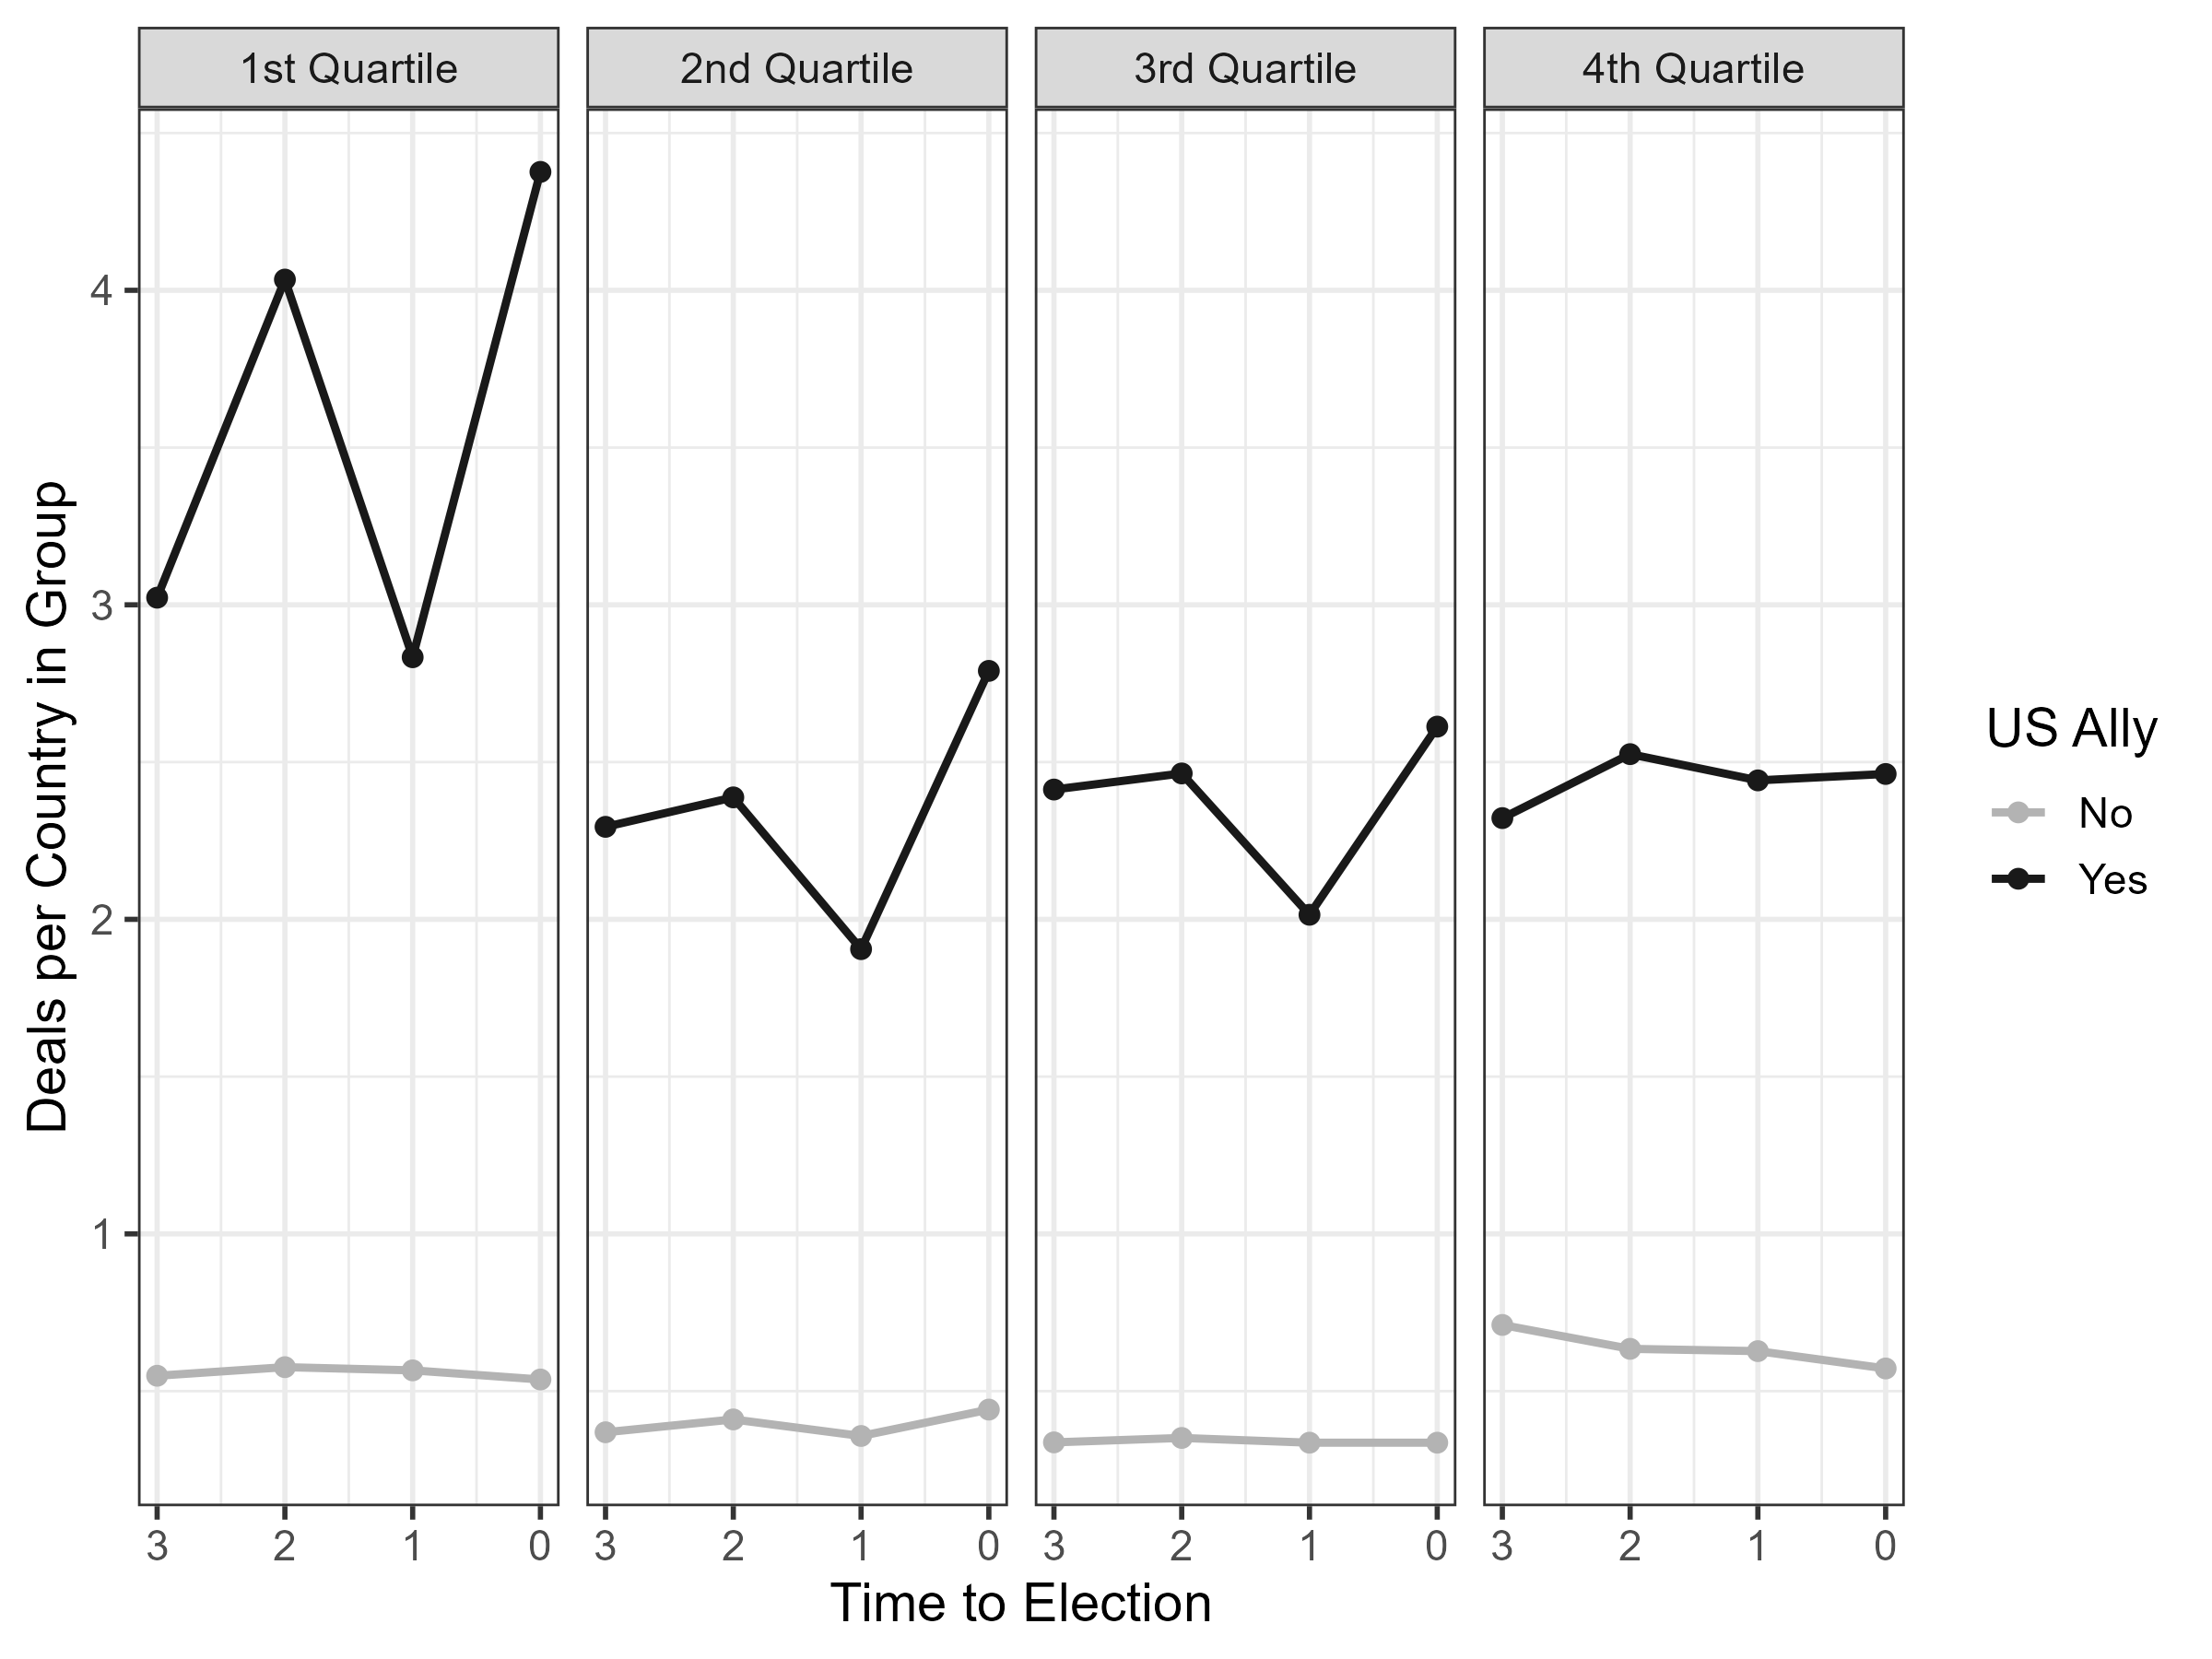
\includegraphics[width=0.95\textwidth]{deals-democ-raw.png}
	\caption{Average arms deals with the United States per country in each quartile of democracy throughout U.S. presidential election cycles. Colors divide states based on whether they are U.S. allies.}
	\label{fig:deals-democ-raw}
\end{figure}


\subsubsection{General Arms Deal Cycles}

In addition to the raw data, arms deal cycles are apparent even without interacting the time to presidential election measure with the autocracy indicator.
I plot predicted arms deals in \autoref{fig:elec-pred-deals}. 
The increase of .05 deals across a presidential election cycle is small but distinguishable from zero. 


\begin{figure}[htpb]
	\centering
		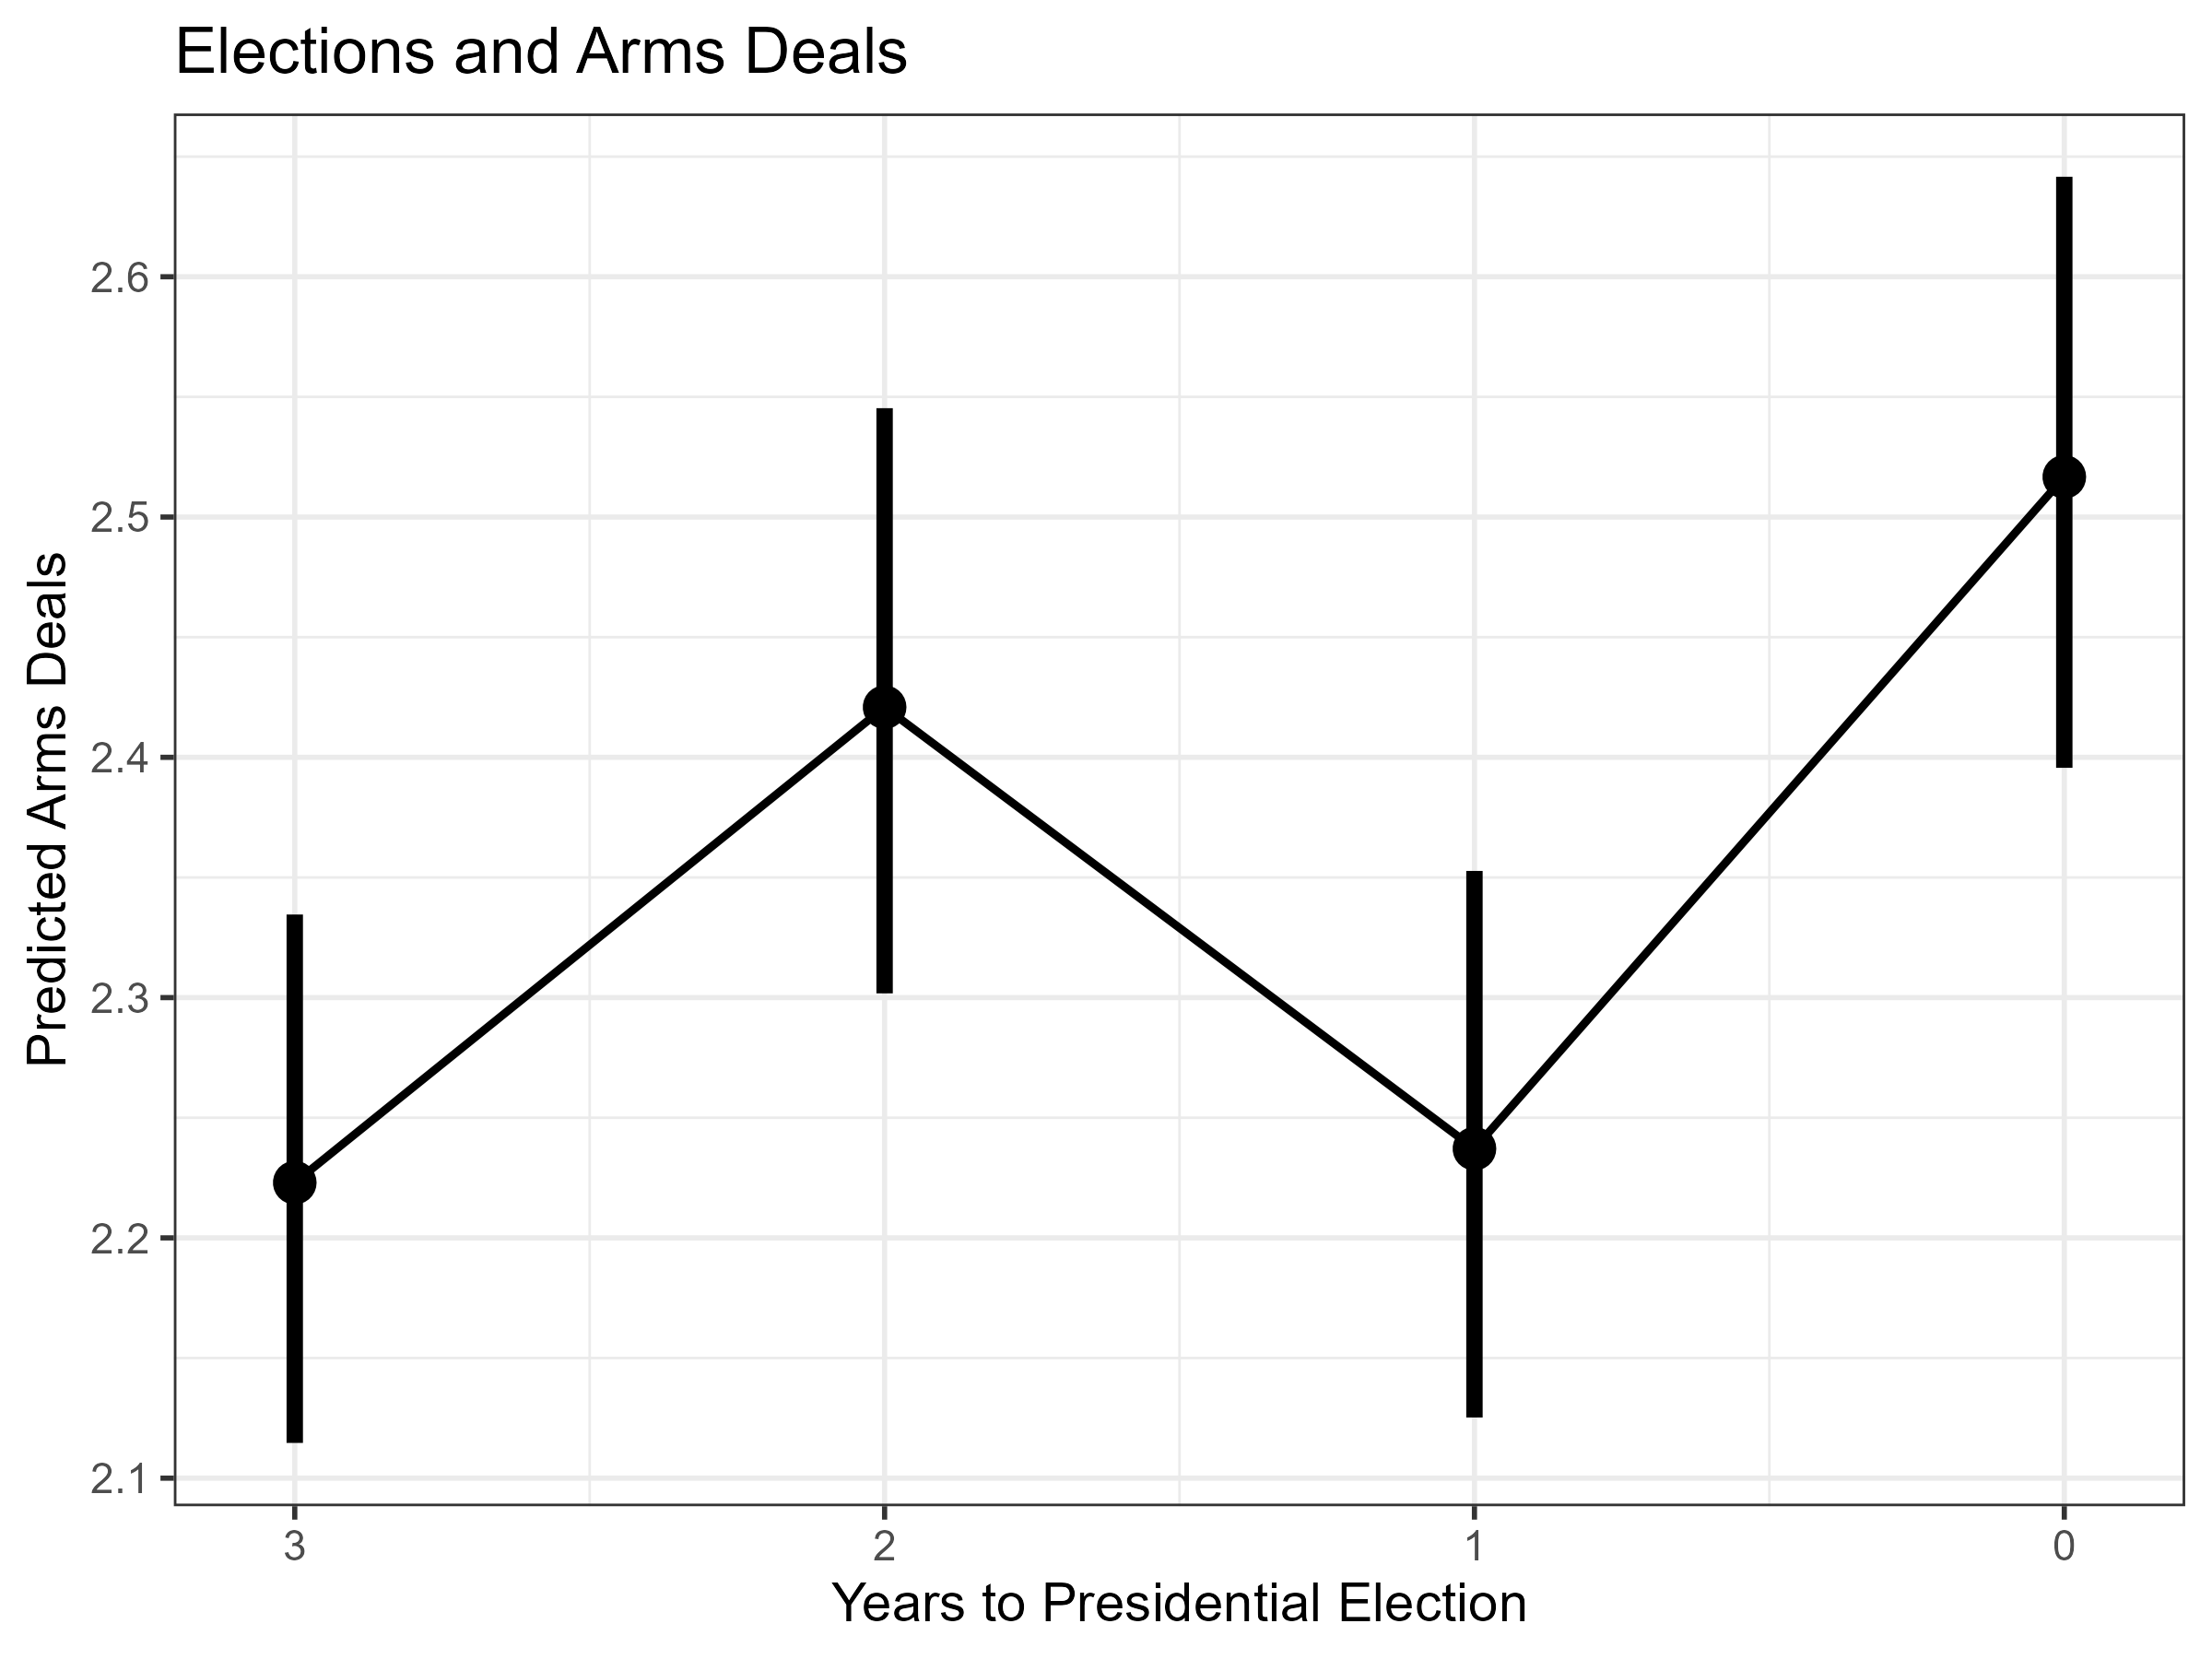
\includegraphics[width=0.95\textwidth]{elec-pred-deals.png}
	\caption{Predicted arms deals by the United States across the presidential election cycle, all else equal. Estimates from a hurdle Poisson model of arms deals between 1950 and 2014. }
	\label{fig:elec-pred-deals}
\end{figure}



\subsection{Alternative Estimators}


The same pattern is also apparent if I use three alternative likelihoods in the model of arms deals, election timing, autocracy and allies. 
While the hurdle Poisson is the most theoretically appropriate specification, linear regression, standard Poisson and zero-inflated Poisson models all give similar inferences.
I plot predicted arms deals across recipient democracy, alliance status and election timing from each of these models in \autoref{fig:deals-pred-ols},  \autoref{fig:deals-pred-pois} and \autoref{fig:deals-pred-zip}. 
All three estimators suggest increasing arms deals for autocratic allies as elections approach, and little change in deals with democratic allies near presidential elections. 


\begin{figure}[htpb]
	\centering
		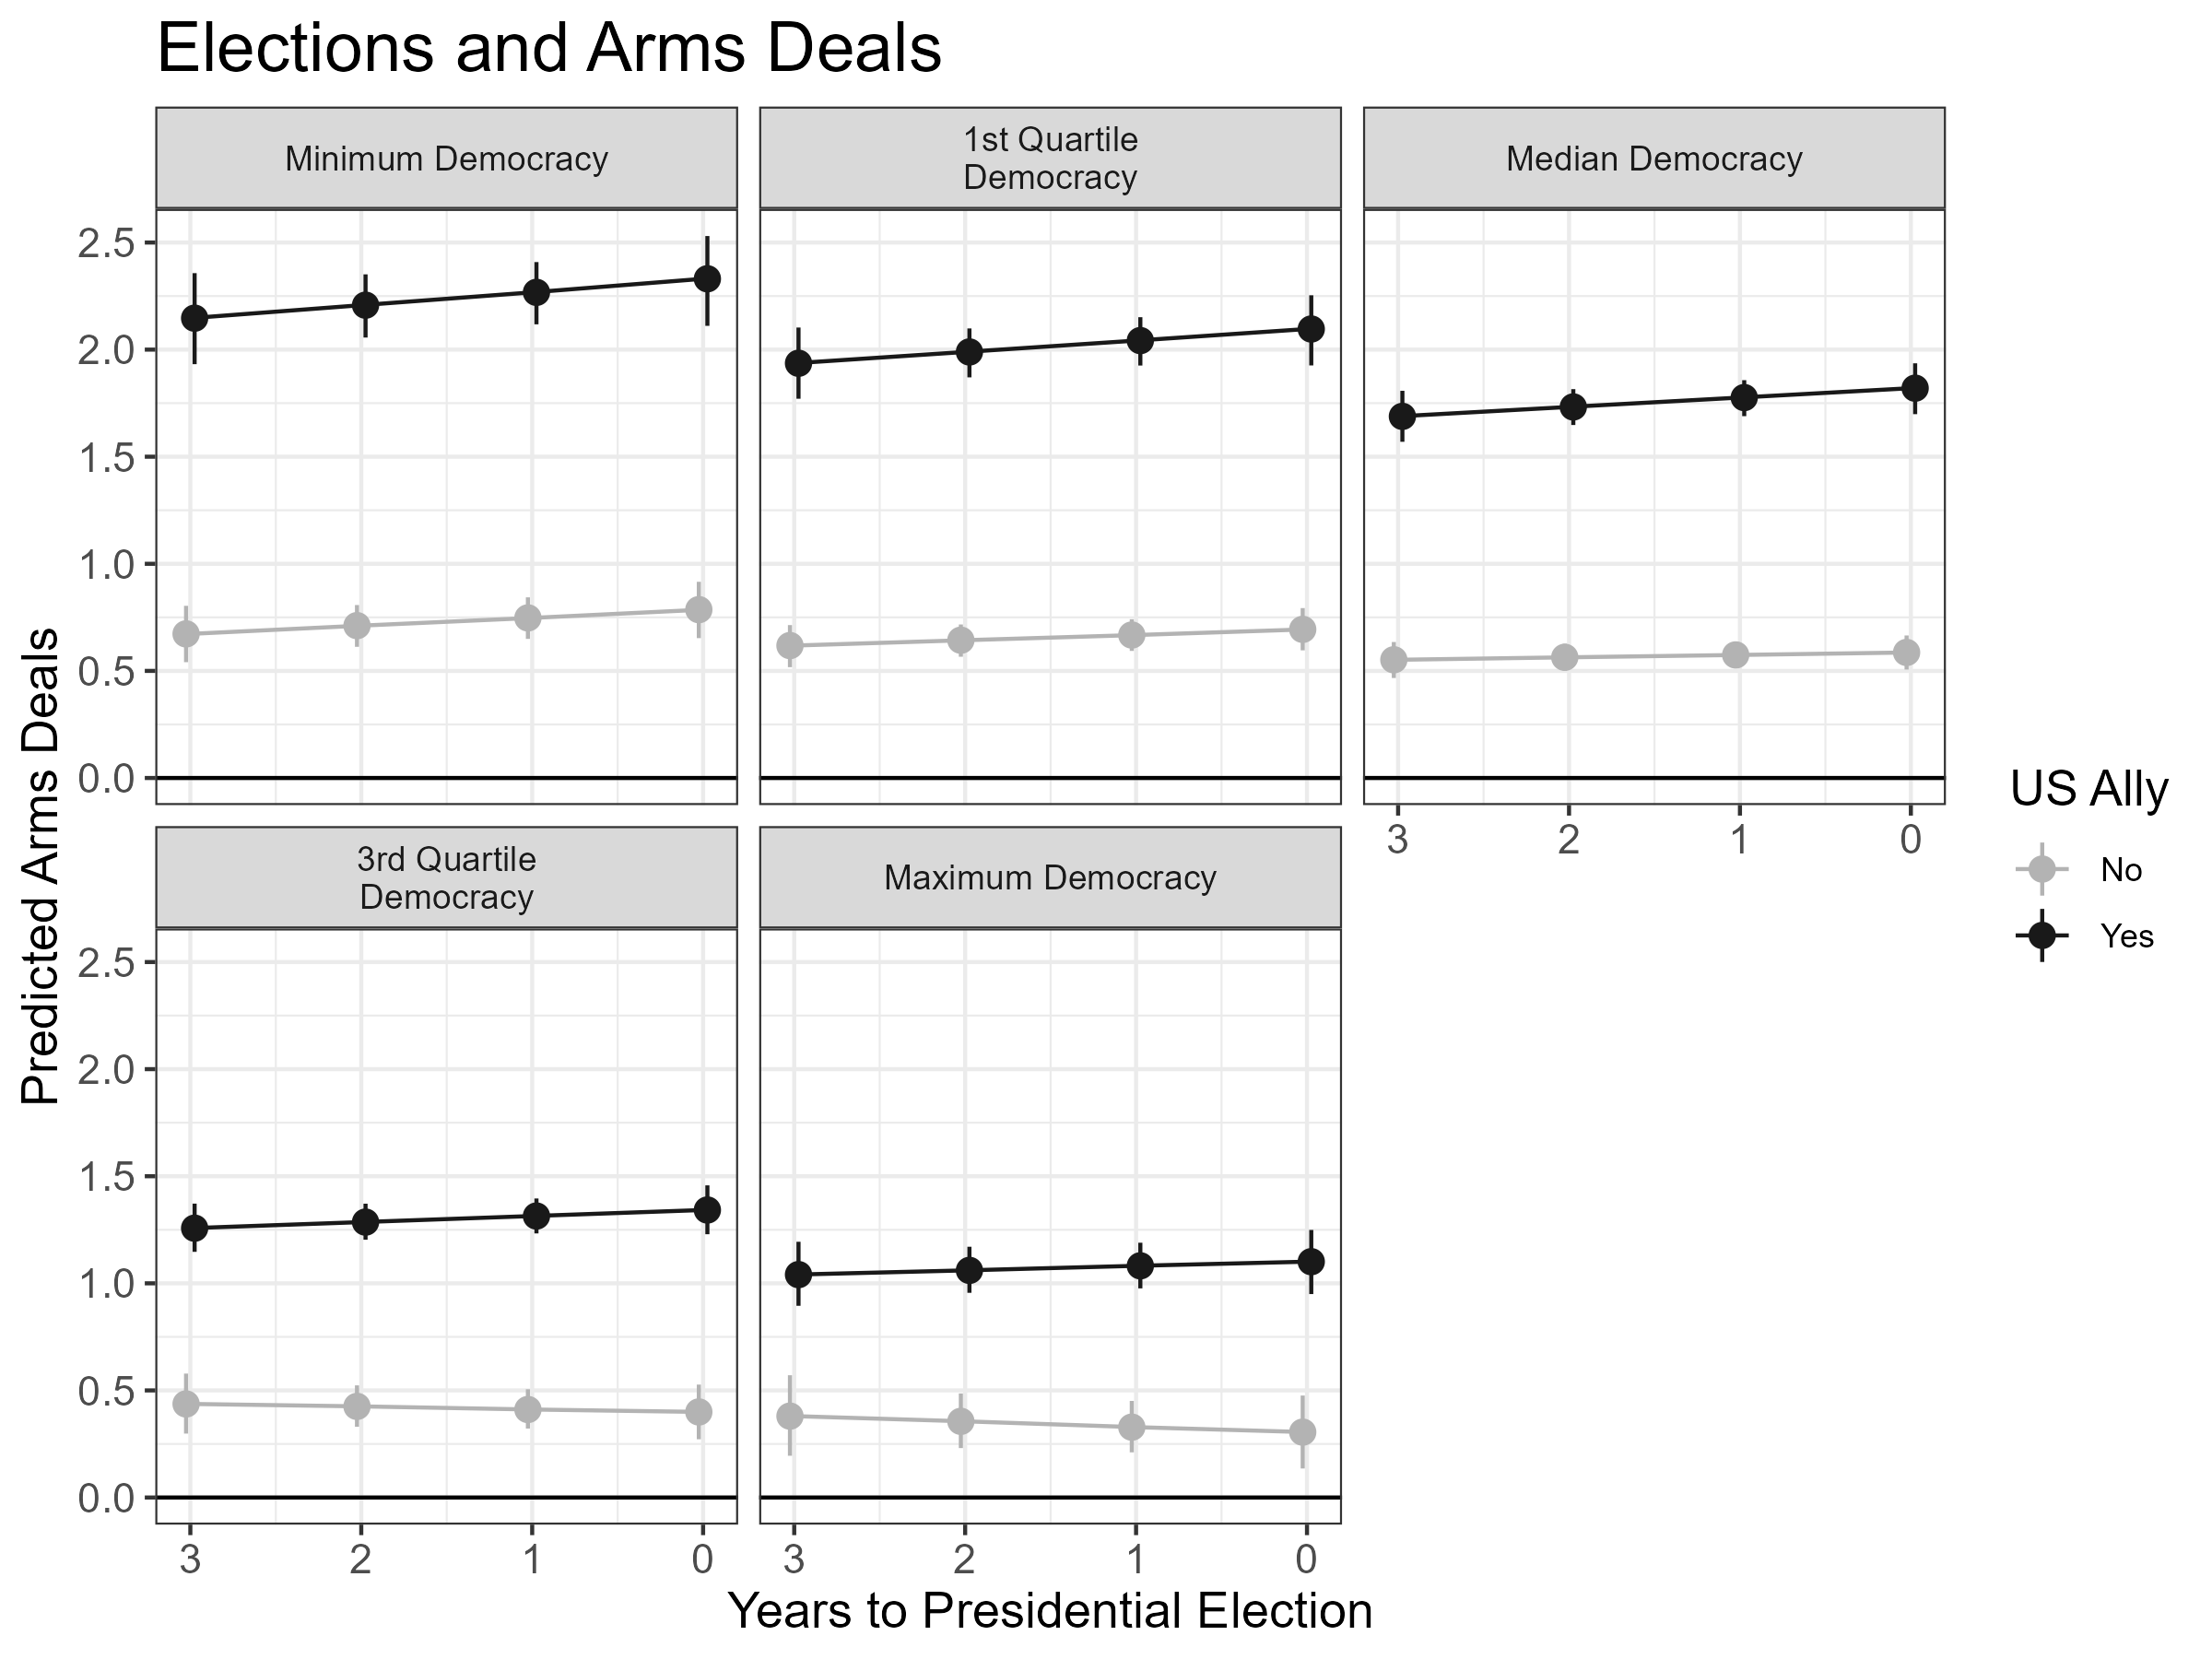
\includegraphics[width=0.95\textwidth]{deals-pred-ols.png}
	\caption{Predicted arms deals between the United States and other states 1950 to 2014 based on presidential election proximity, democracy, and security alliances, based on a linear regression model. Points mark the estimates and error bars summarize the 90\% credible interval.}
	\label{fig:deals-pred-ols}
\end{figure}



\begin{figure}[htpb]
	\centering
		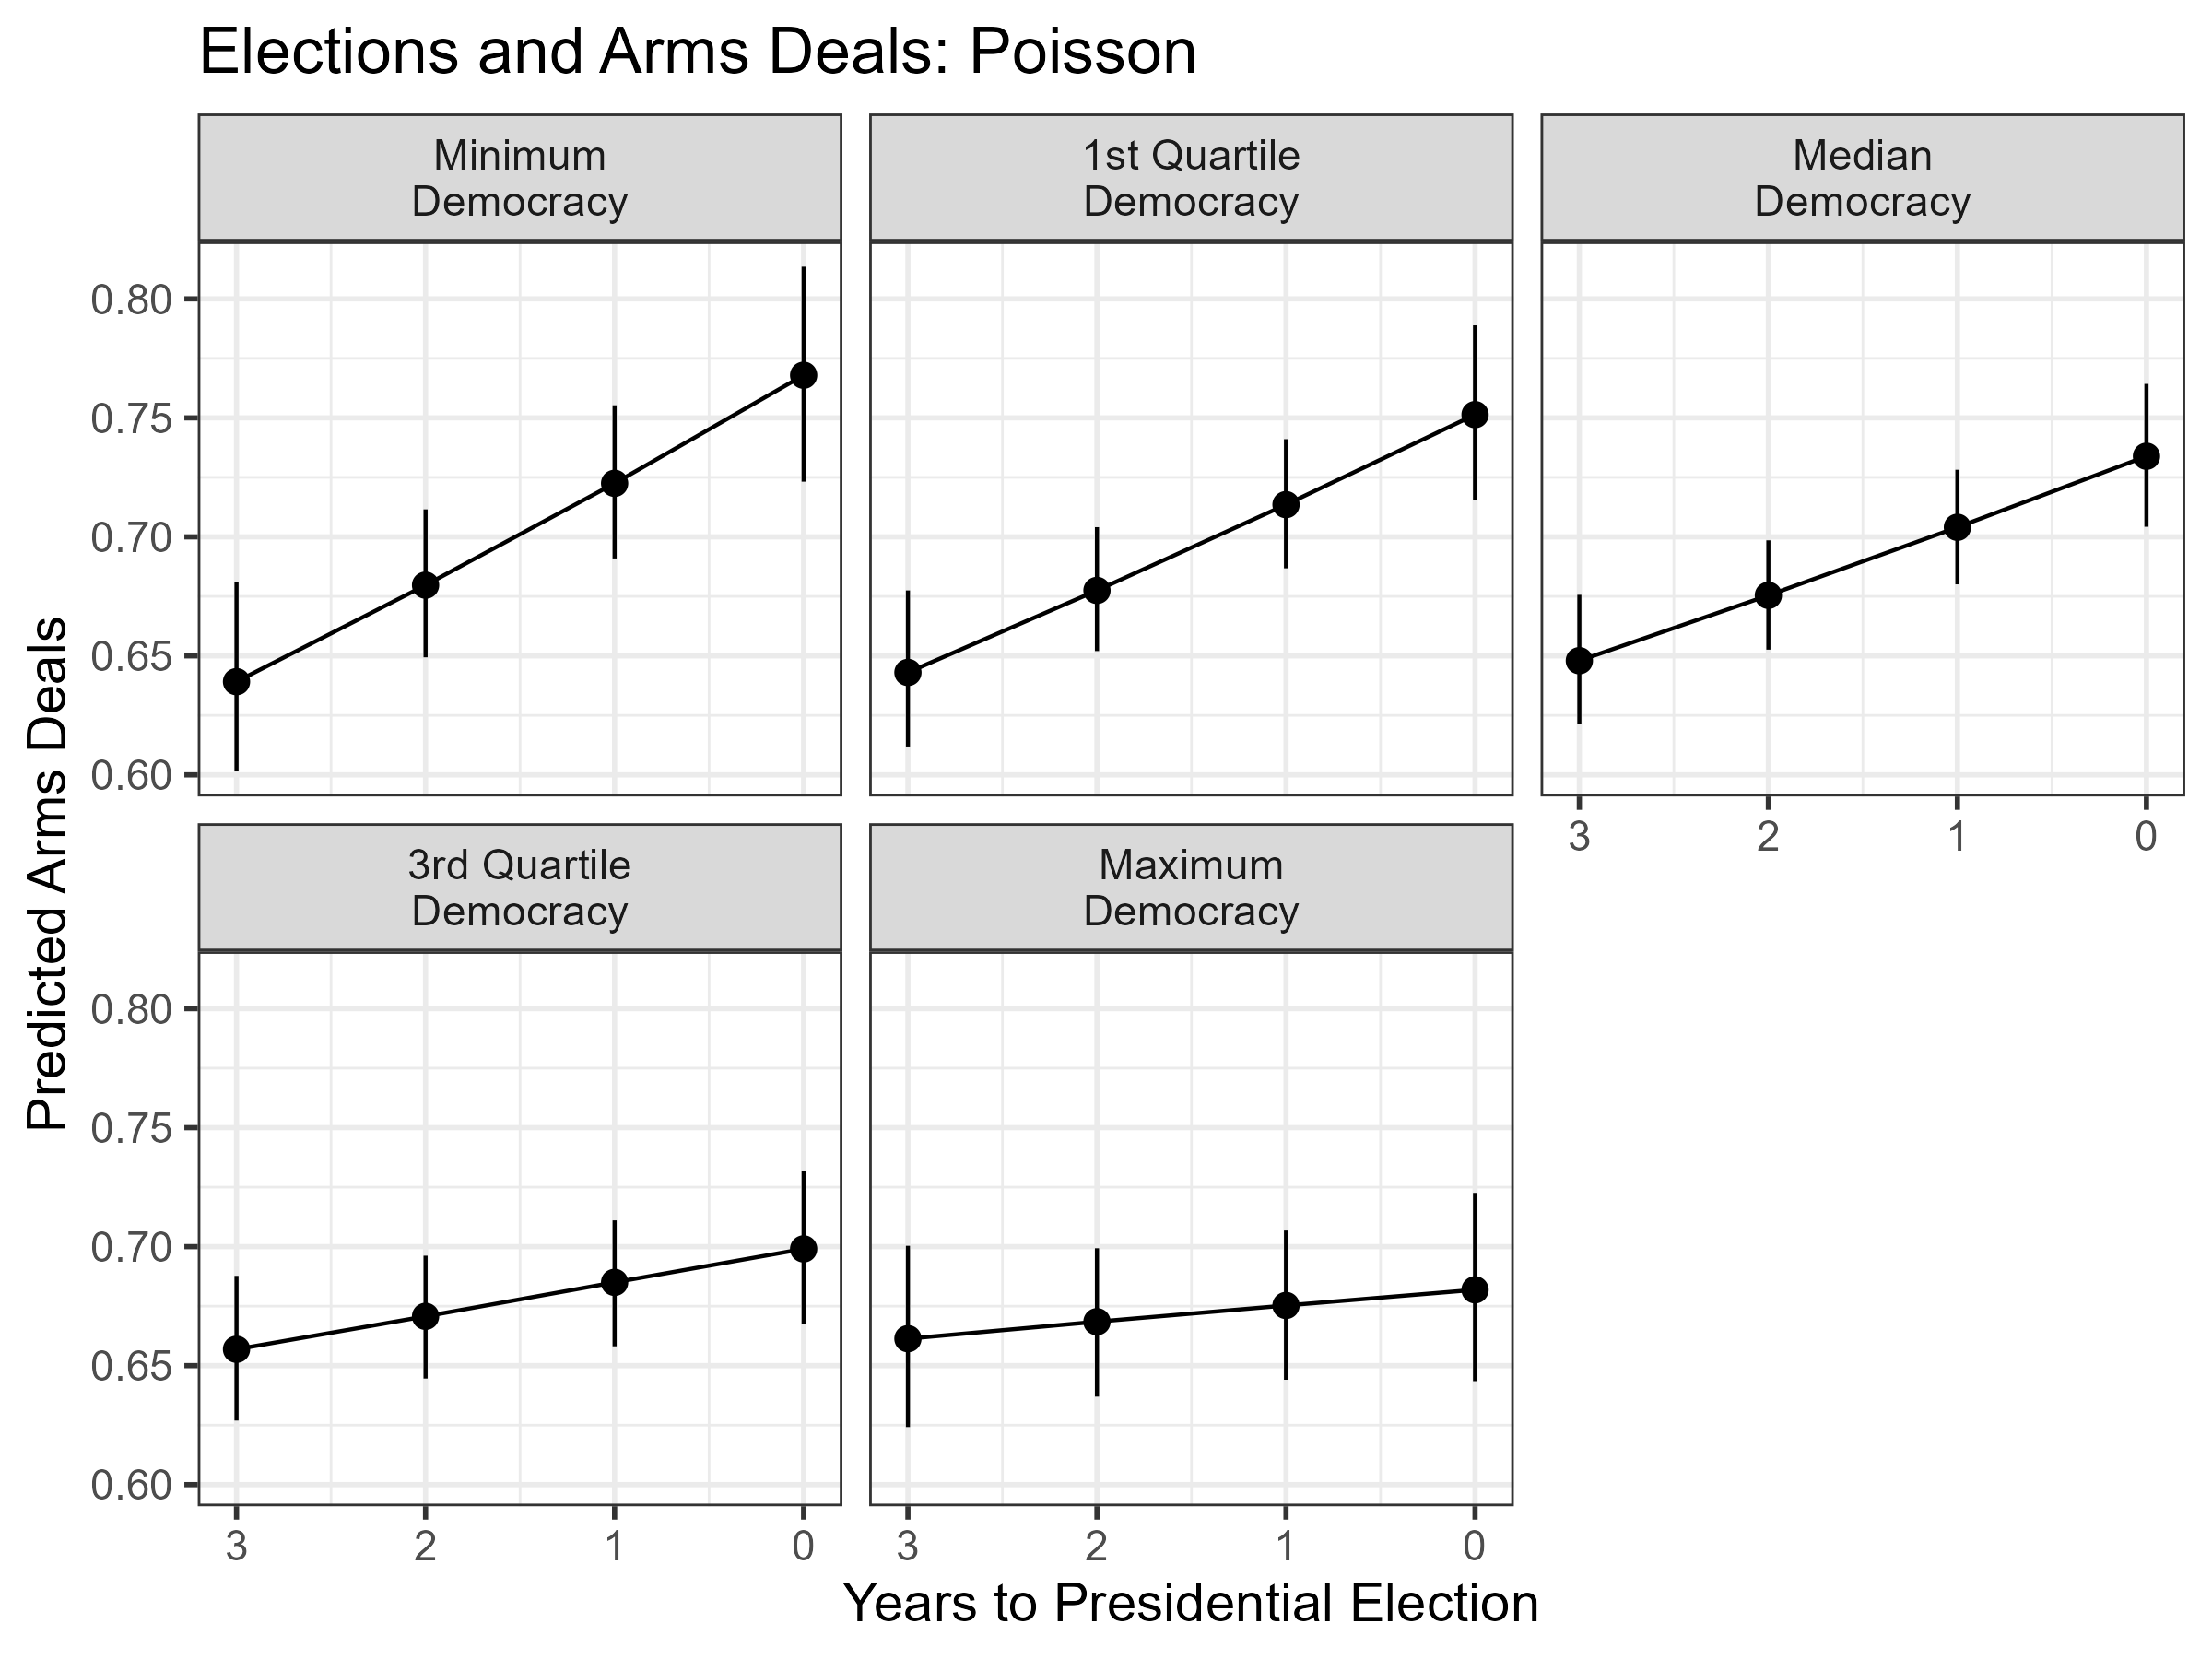
\includegraphics[width=0.95\textwidth]{deals-pred-pois.png}
	\caption{Predicted arms deals between the United States and other states 1950 to 2014 based on presidential election proximity, democracy, and security alliances, based on a Poisson model. Points mark the estimates and error bars summarize the 90\% credible interval.}
	\label{fig:deals-pred-pois}
\end{figure}



\begin{figure}[htpb]
	\centering
		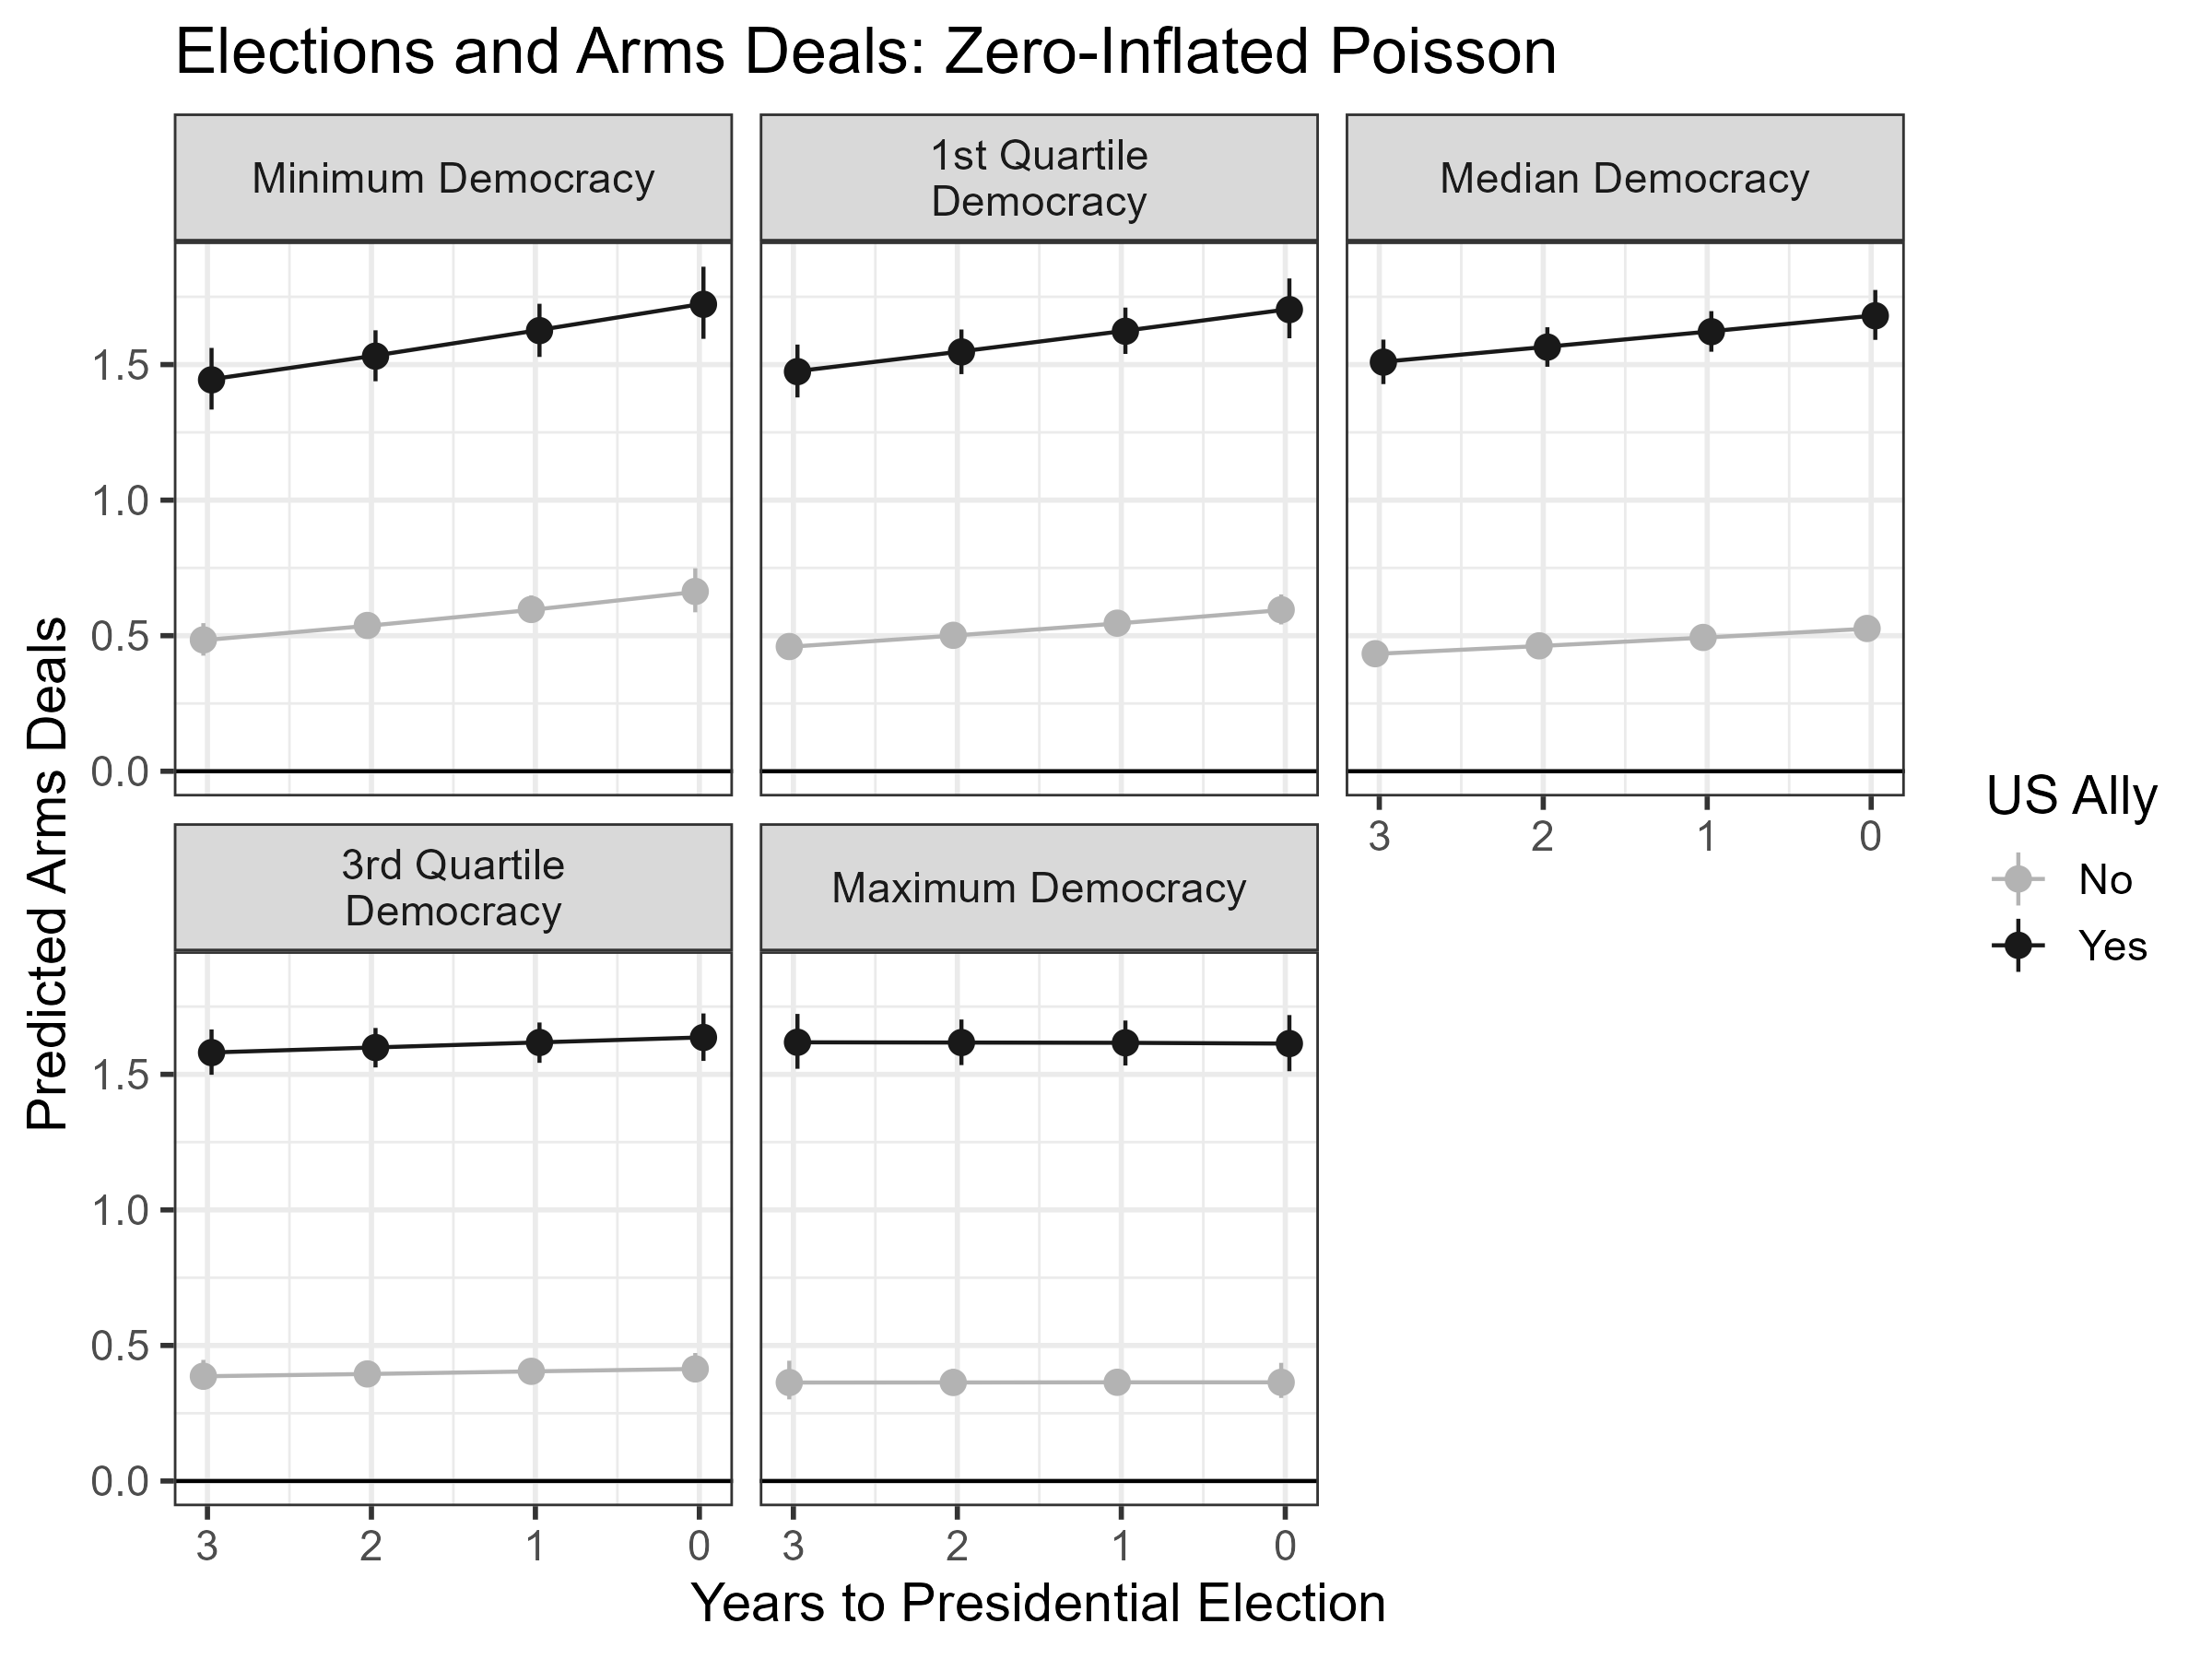
\includegraphics[width=0.95\textwidth]{deals-pred-zip.png}
	\caption{{Predicted arms deals between the United States and other states 1950 to 2014 based on presidential election proximity, democracy, and security alliances, based on a zero-inflated Poisson model. Points mark the estimates and error bars summarize the 90\% credible interval.}}
	\label{fig:deals-pred-zip}
\end{figure}


\subsection{Posterior Predictive Checks}


This final check shows the predictive performance of the hurdle Poisson model, relative to a negative binomial likelihood. 
While neither model captures the lumpy outcome distribution, the hurdle Poisson is much better 
First, I show the posterior predictive check for the hurdle Poisson in \autoref{fig:pp-check-deals}. 


Both \autoref{fig:pp-check-deals} and \autoref{fig:nb-pp-check} are rootograms, which plot expected counts against observed counts. 
In both figures, the line gives the expected counts based on the model, and the bars mark observed counts. 
Bars that exceed zero are counts the model under predicts, while bars above zero are underpredicted. 
As a result, the hurdle Poisson predicts zero values well, underpredicts some large values, and overpredicts a few small values. 



\begin{figure}[htpb]
	\centering
		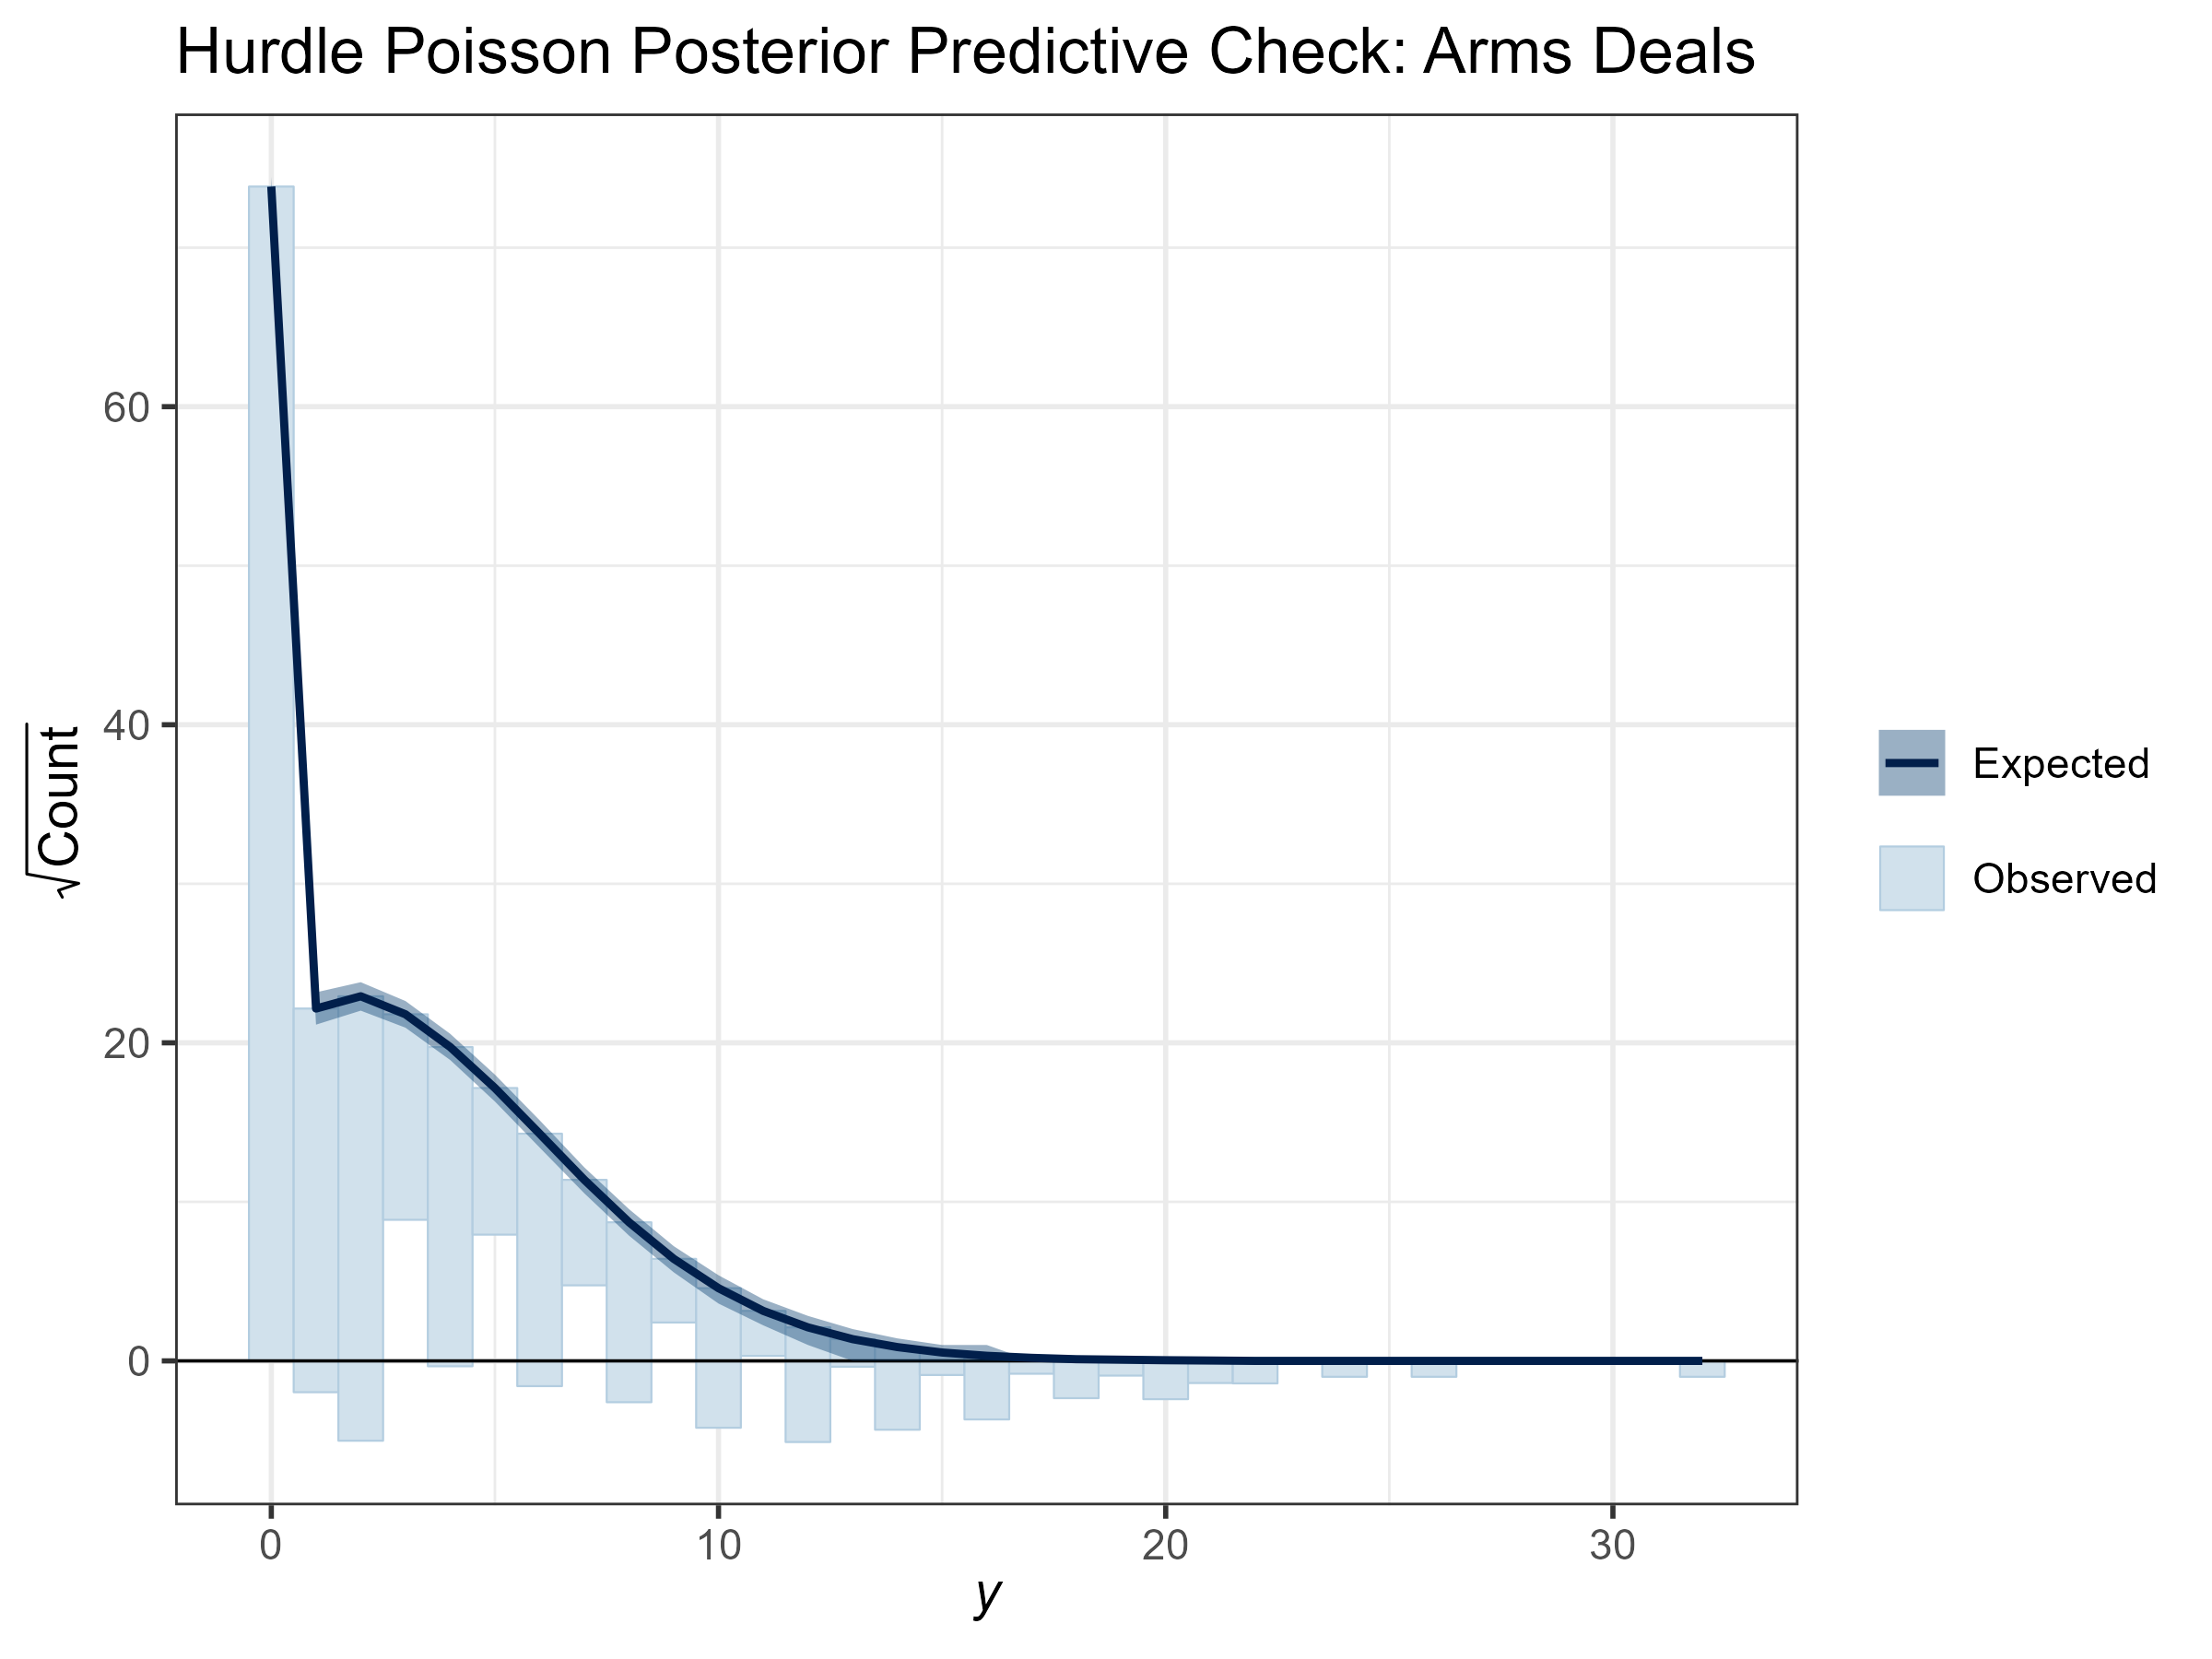
\includegraphics[width=0.95\textwidth]{pp-check-deals.png}
	\caption{Posterior predictive check of the hurdle Poisson model of US arms deals. In this rootogram, the fitted line gives the expected counts and bars show the observed distribution.}
	\label{fig:pp-check-deals}
\end{figure}


Relative to the hurdle, a regular Poisson model under-predicts zeros, as \autoref{fig:pois-pp-check} demonstrates. 
This also moves the model fit and reduces predictive accuracy for non-zero deals. 


\begin{figure}[htpb]
	\centering
		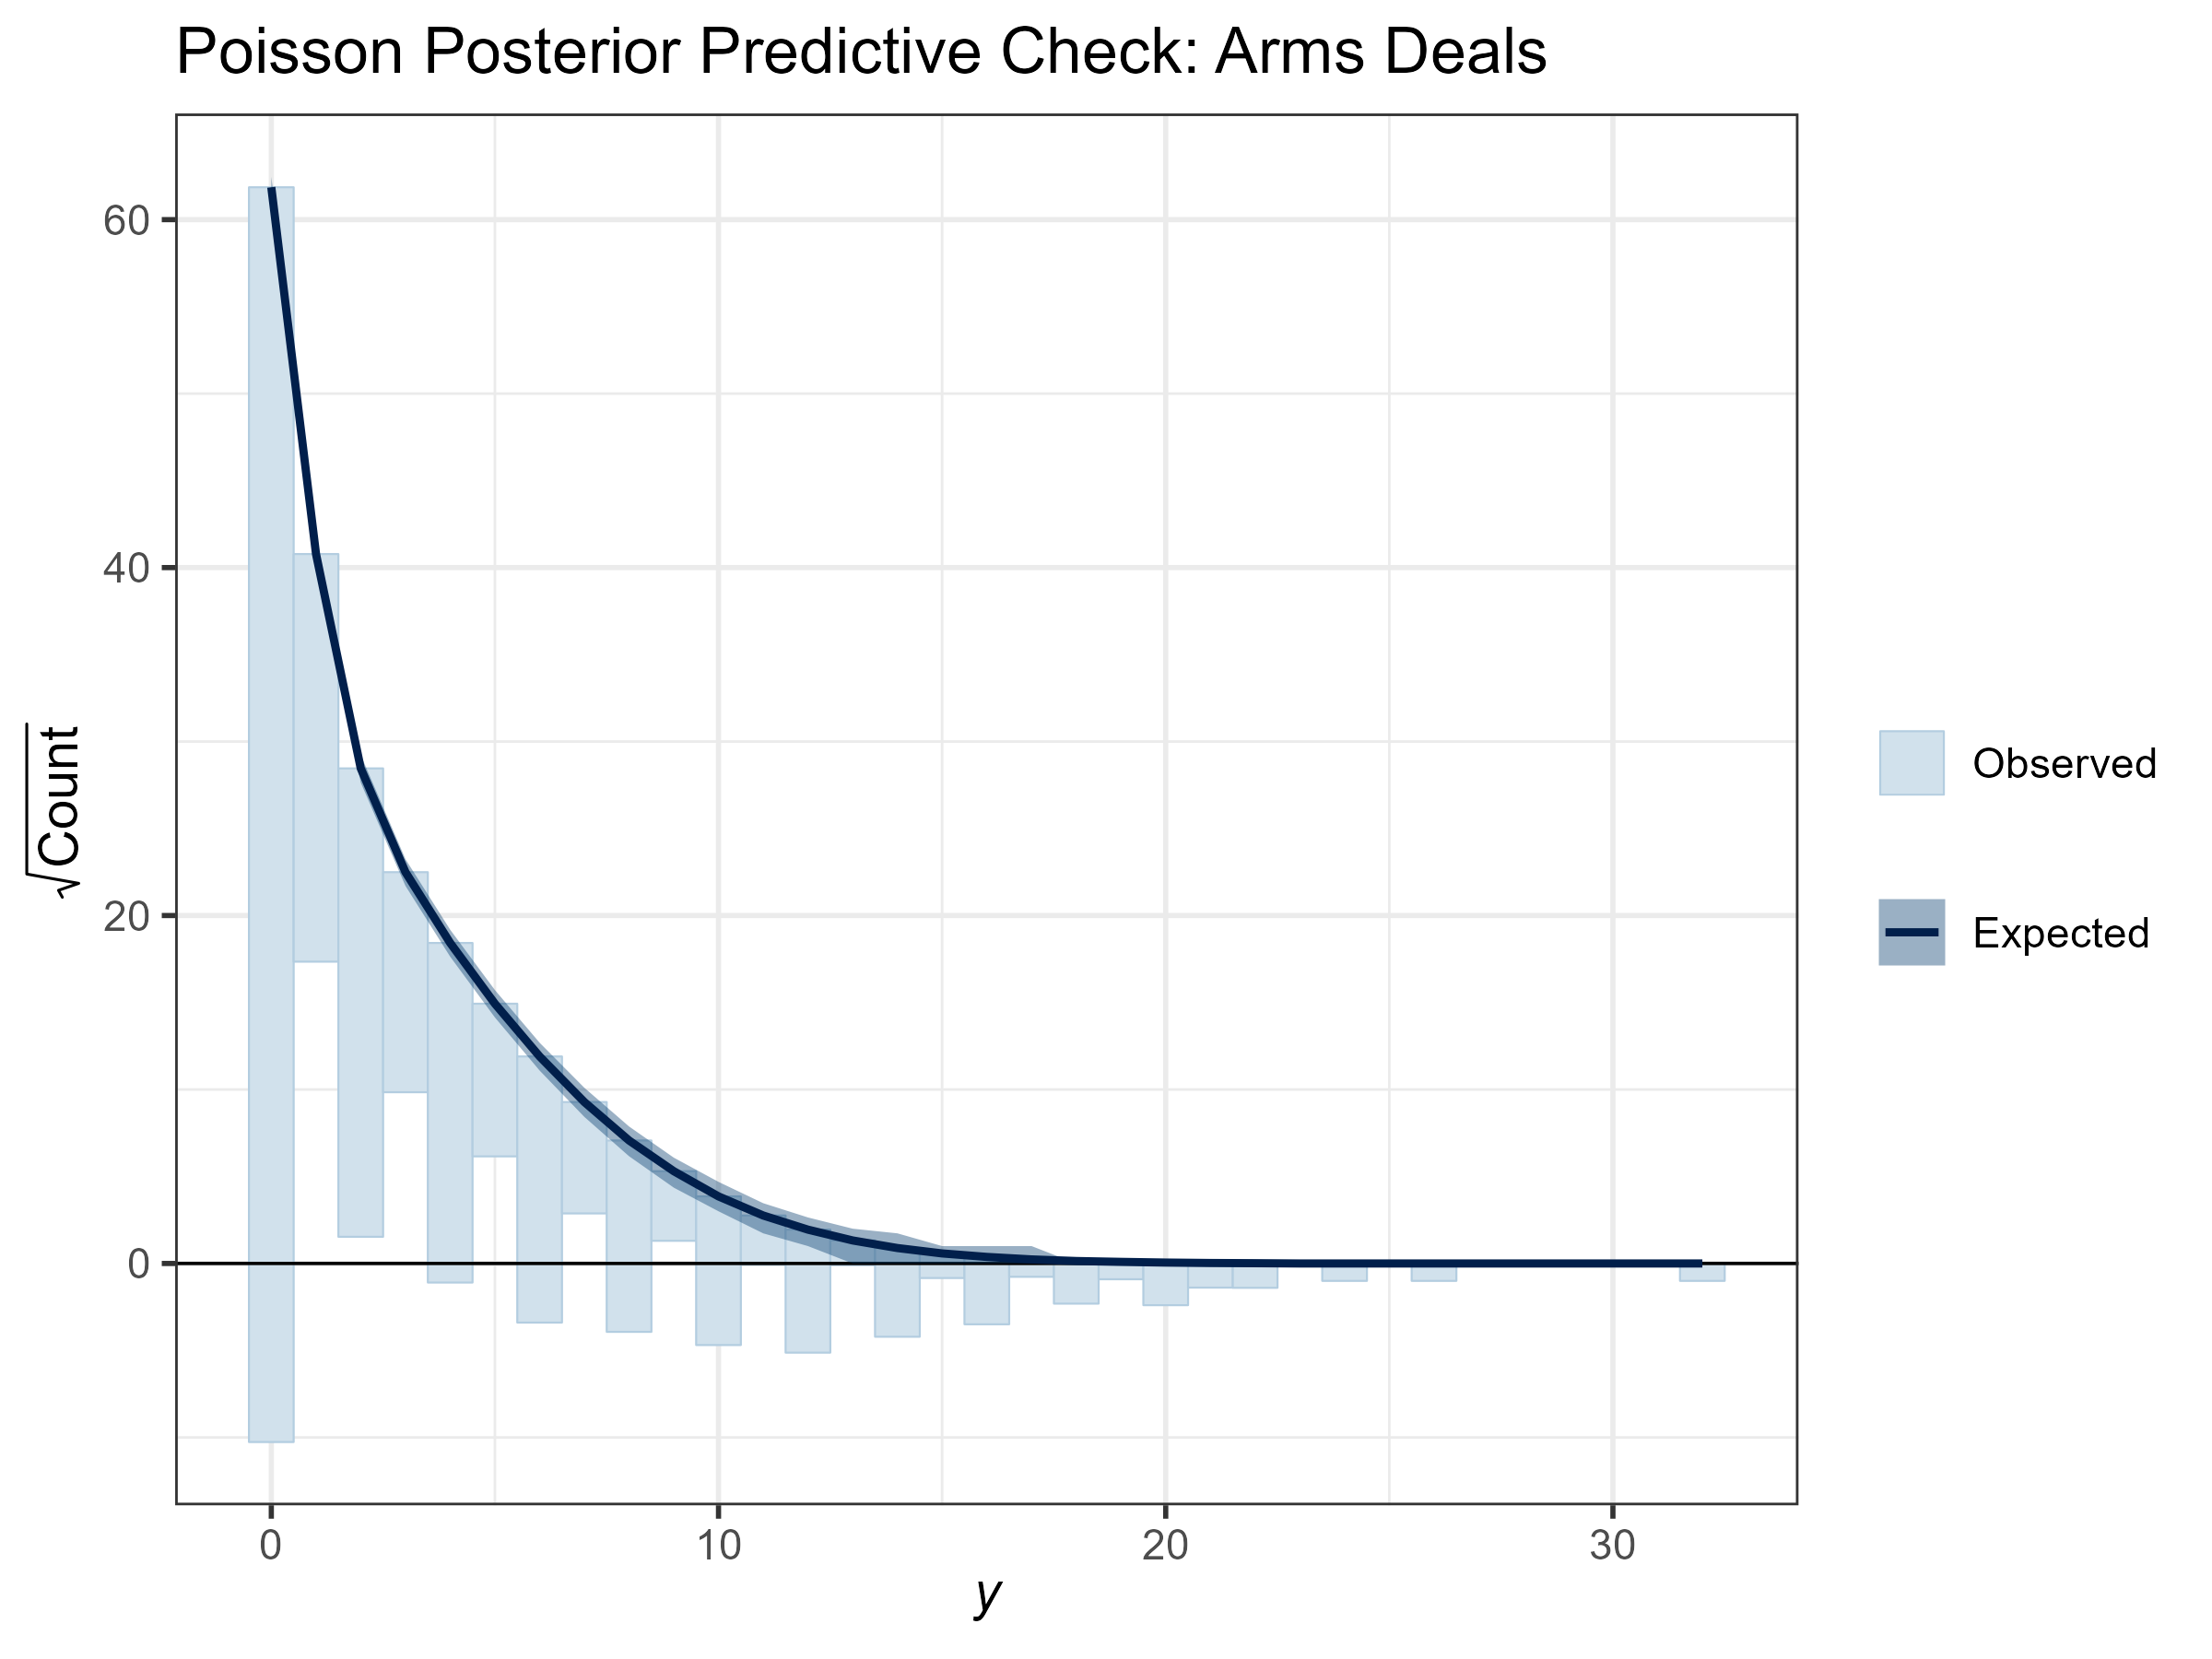
\includegraphics[width=0.95\textwidth]{pois-pp-check.png}
	\caption{Posterior predictive check of a Poisson model of US arms deals. In this rootogram, the fitted line gives the expected counts and bars show the observed distribution.}
	\label{fig:pois-pp-check}
\end{figure}


While the lumpy distribution of deals complicates predictions with a Poisson likelihood, a negative binomial likelihood fits poorly. 
As \autoref{fig:nb-pp-check} demonstrates, the extra variance in a negative binomial results in underpredicting almost all observed values, and some predictions that are far above the range of the observed data. 
This is why I rely on models with a Poisson likelihood and do not report negative binomial estimates. 


\begin{figure}[htpb]
	\centering
		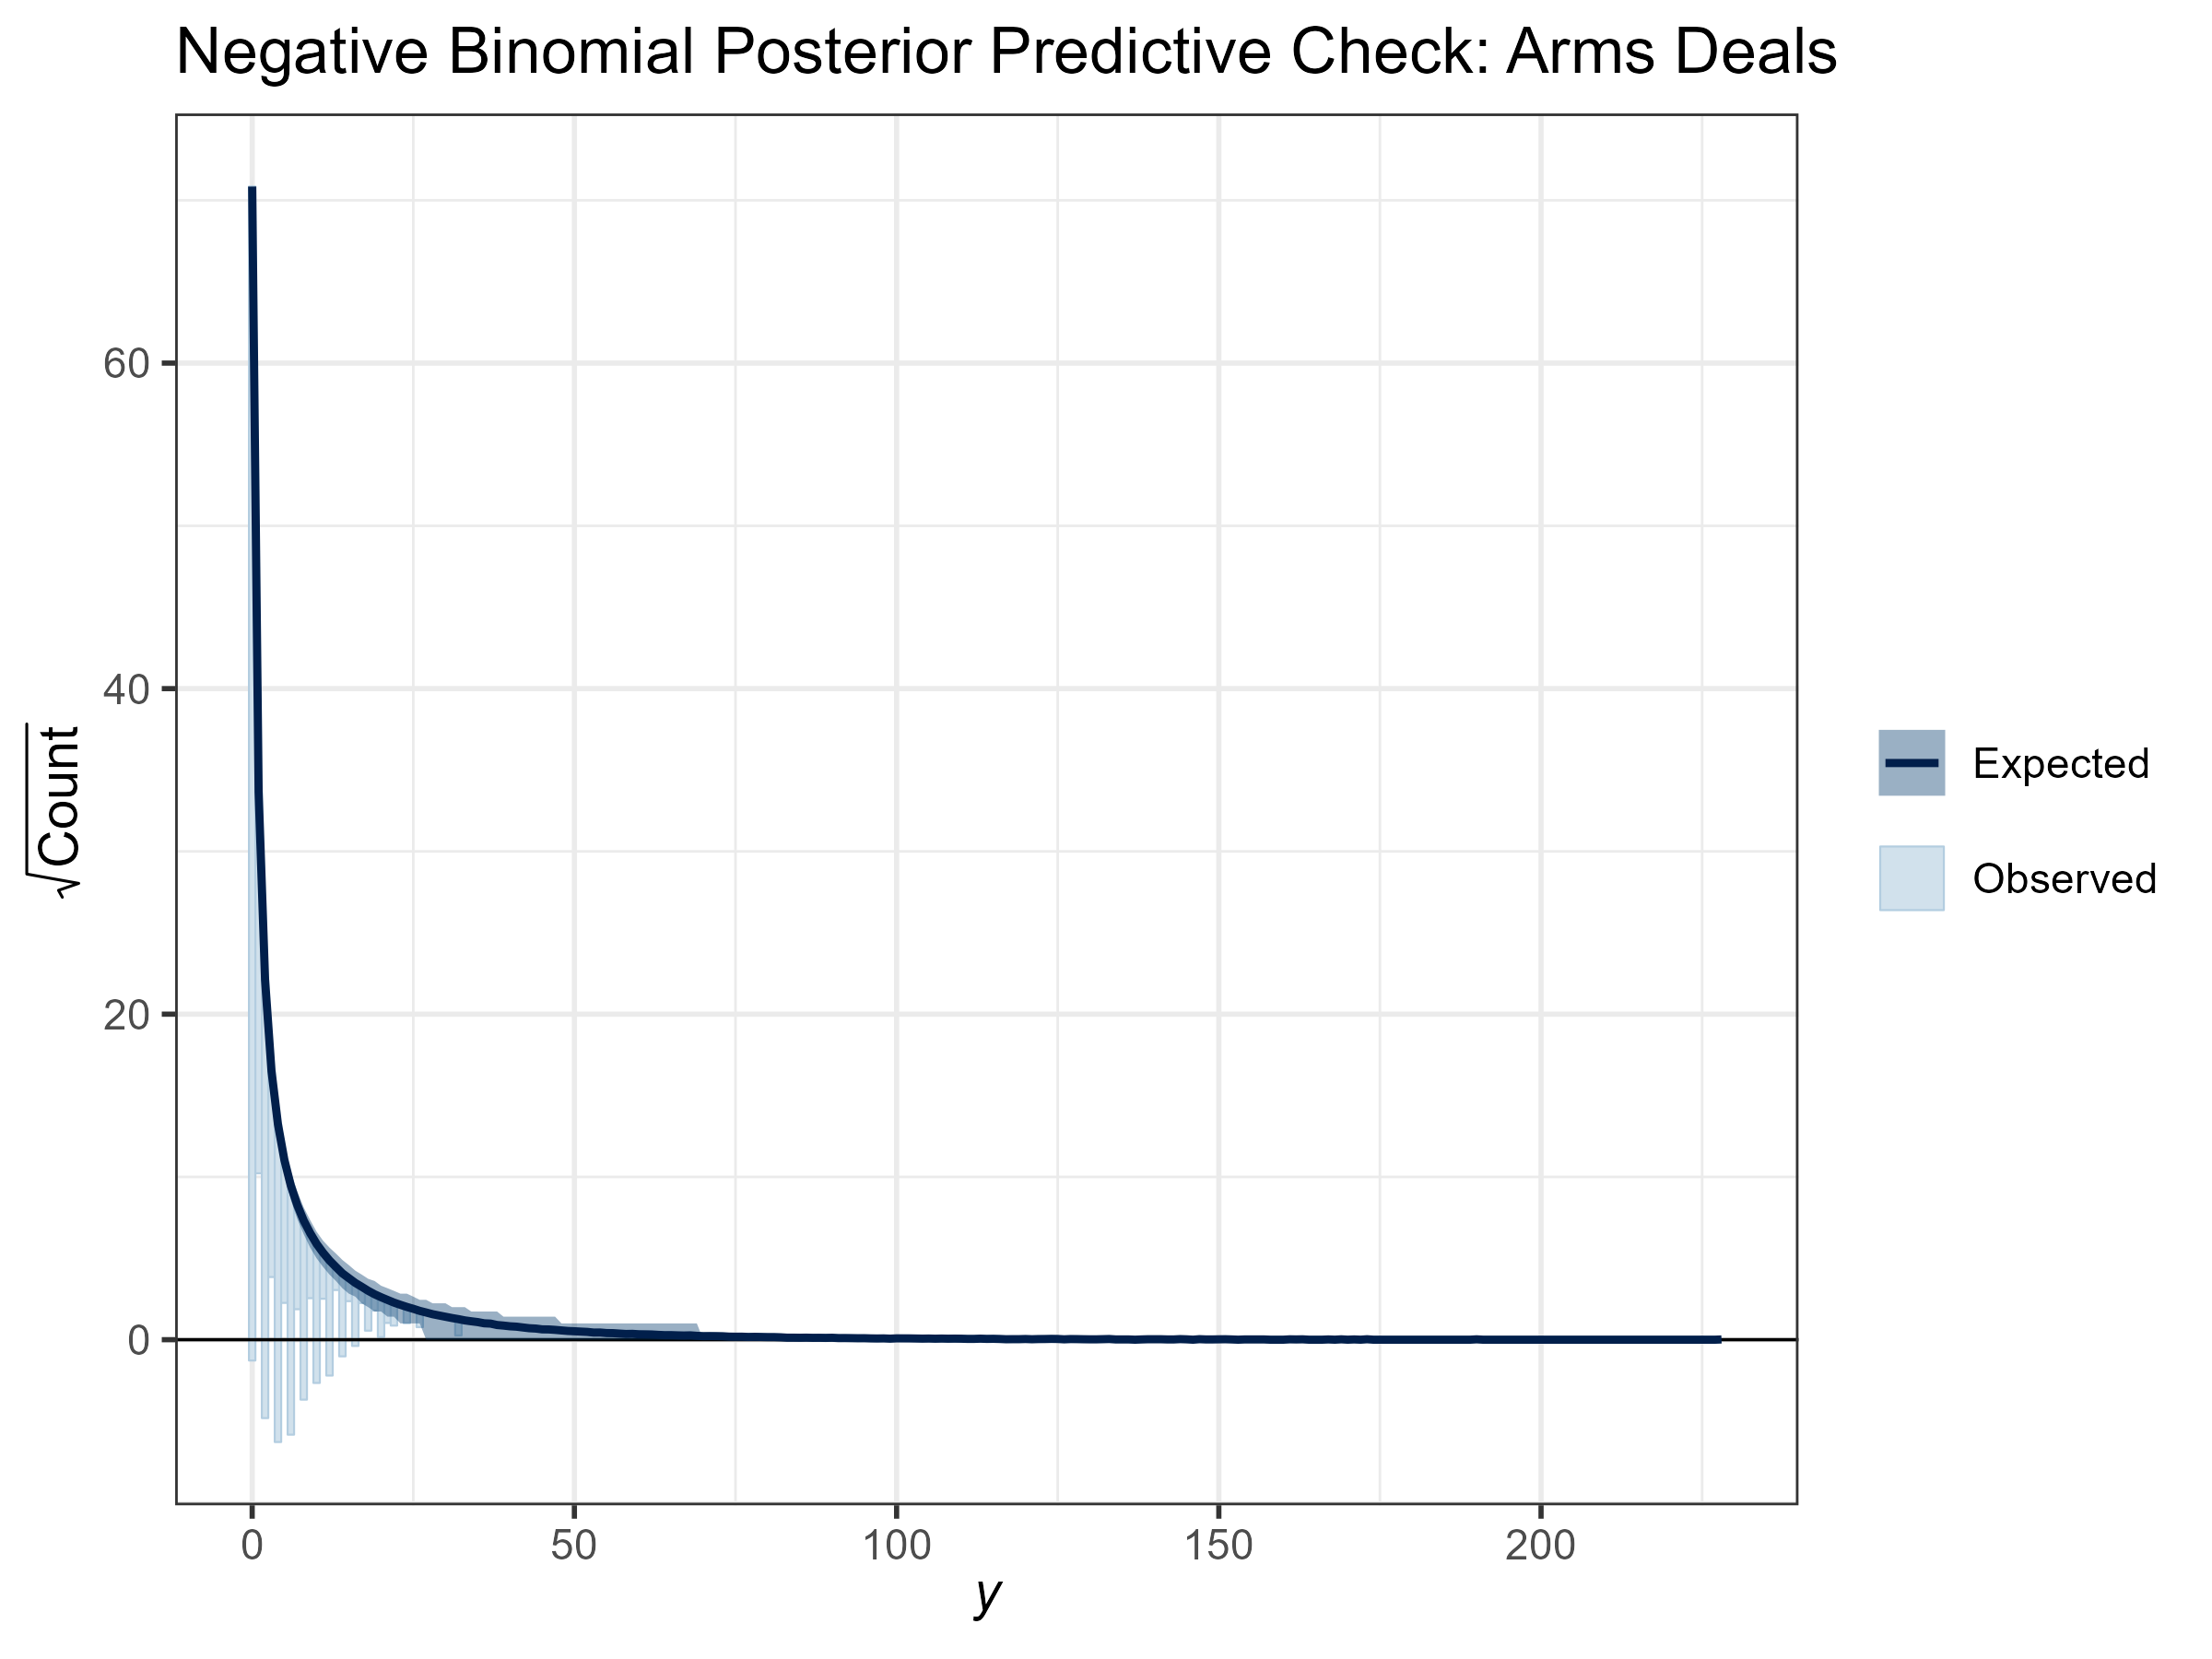
\includegraphics[width=0.95\textwidth]{nb-pp-check.png}
	\caption{Posterior predictive check of a negative binomial model of US arms deals. In this rootogram, the fitted line gives the expected counts and bars show the observed distribution.}
	\label{fig:nb-pp-check}
\end{figure}


\section{Contracts Model Checks} 

This section checks the second analysis, which examines the interaction between arms deals and contract awards in the 50 states. 
First, I present additional estimates from the ordered beta regression- the state varying intercepts and lagged dependent variables. 
I then show that student-t and hurdle log-normal models of defense contract changes and levels also suggest that arms deals increase contract awards to swing states. 


\subsection{Additional Estimates}


\autoref{fig:state-pars} presents estimates from the ordered beta regression with transformed contracts. 
There is wide variation in contracting levels and temporal dependence across states. 
States with higher contracting levels also have more consistent temporal autocorrelation in contracts, while states such as North Dakota receive occasional arms contracts and thus have little temporal dependence. 

\begin{figure}[htpb]
	\centering
		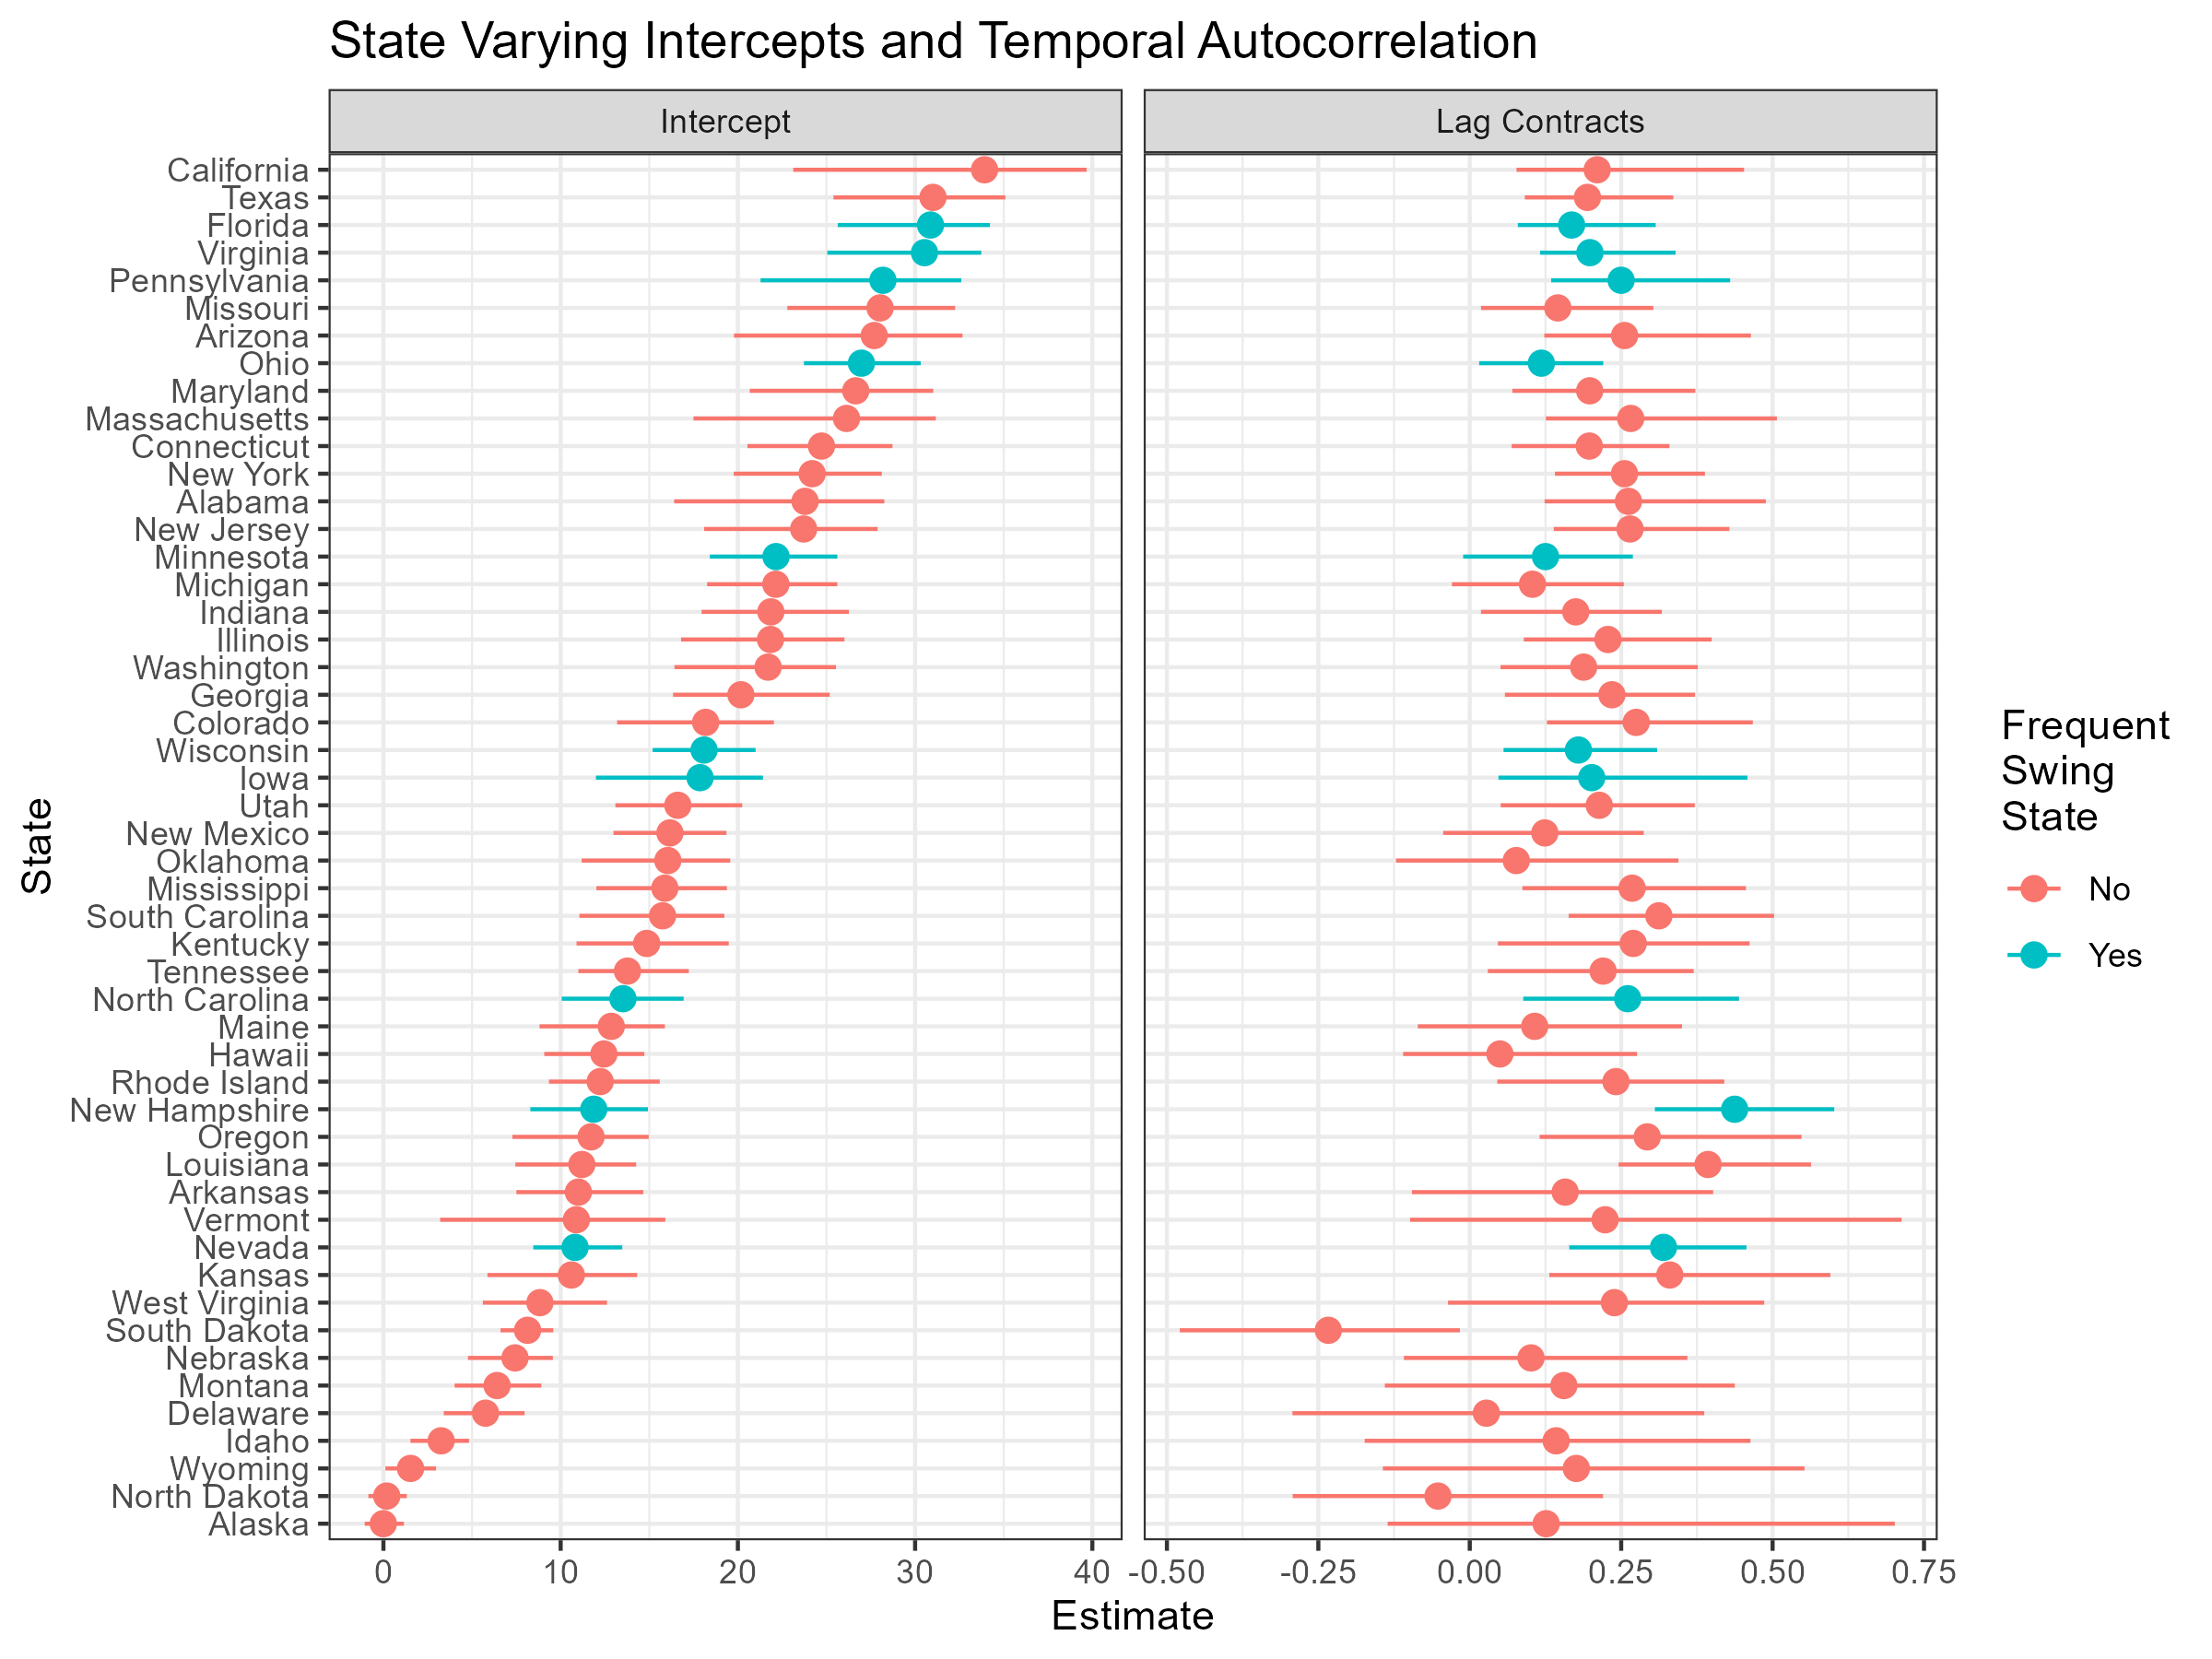
\includegraphics[width=0.95\textwidth]{state-pars.png}
	\caption{Estimated state intercept and temporal autocorrelation from ordered beta regression of transformed defense contracts in US states, 2001-2020. Estimates ordered by the magnitude of the varying intercept. Error bars summarize the 90\% credible interval.}
	\label{fig:state-pars}
\end{figure}


\subsection{Alternative Estimators}

This section checks the results in the manuscript by adjusting the outcome measurement and estimation strategy in two ways.\footnote{All models estimated with brms \citep{Buerkner2017}.} 
First, I do not transform the contracts measure in any way, and fit a log-normal hurdle model, which assumes that the outcome 
This approach does not model state-year observations with zero contracts well, but it fits non-zero contracts well. 
As the top panel of \autoref{fig:me-deals-check} shows, the interaction between arms deals and swing state status is almost entirely positive.
At the same time, the association between deals and the level of contracts outside of swing states is almost entirely negative. 
This latter estimate is not part of the argument, and may be the result of difficulties accounting for zeros. 
 

\begin{figure}[htpb]
	\centering
		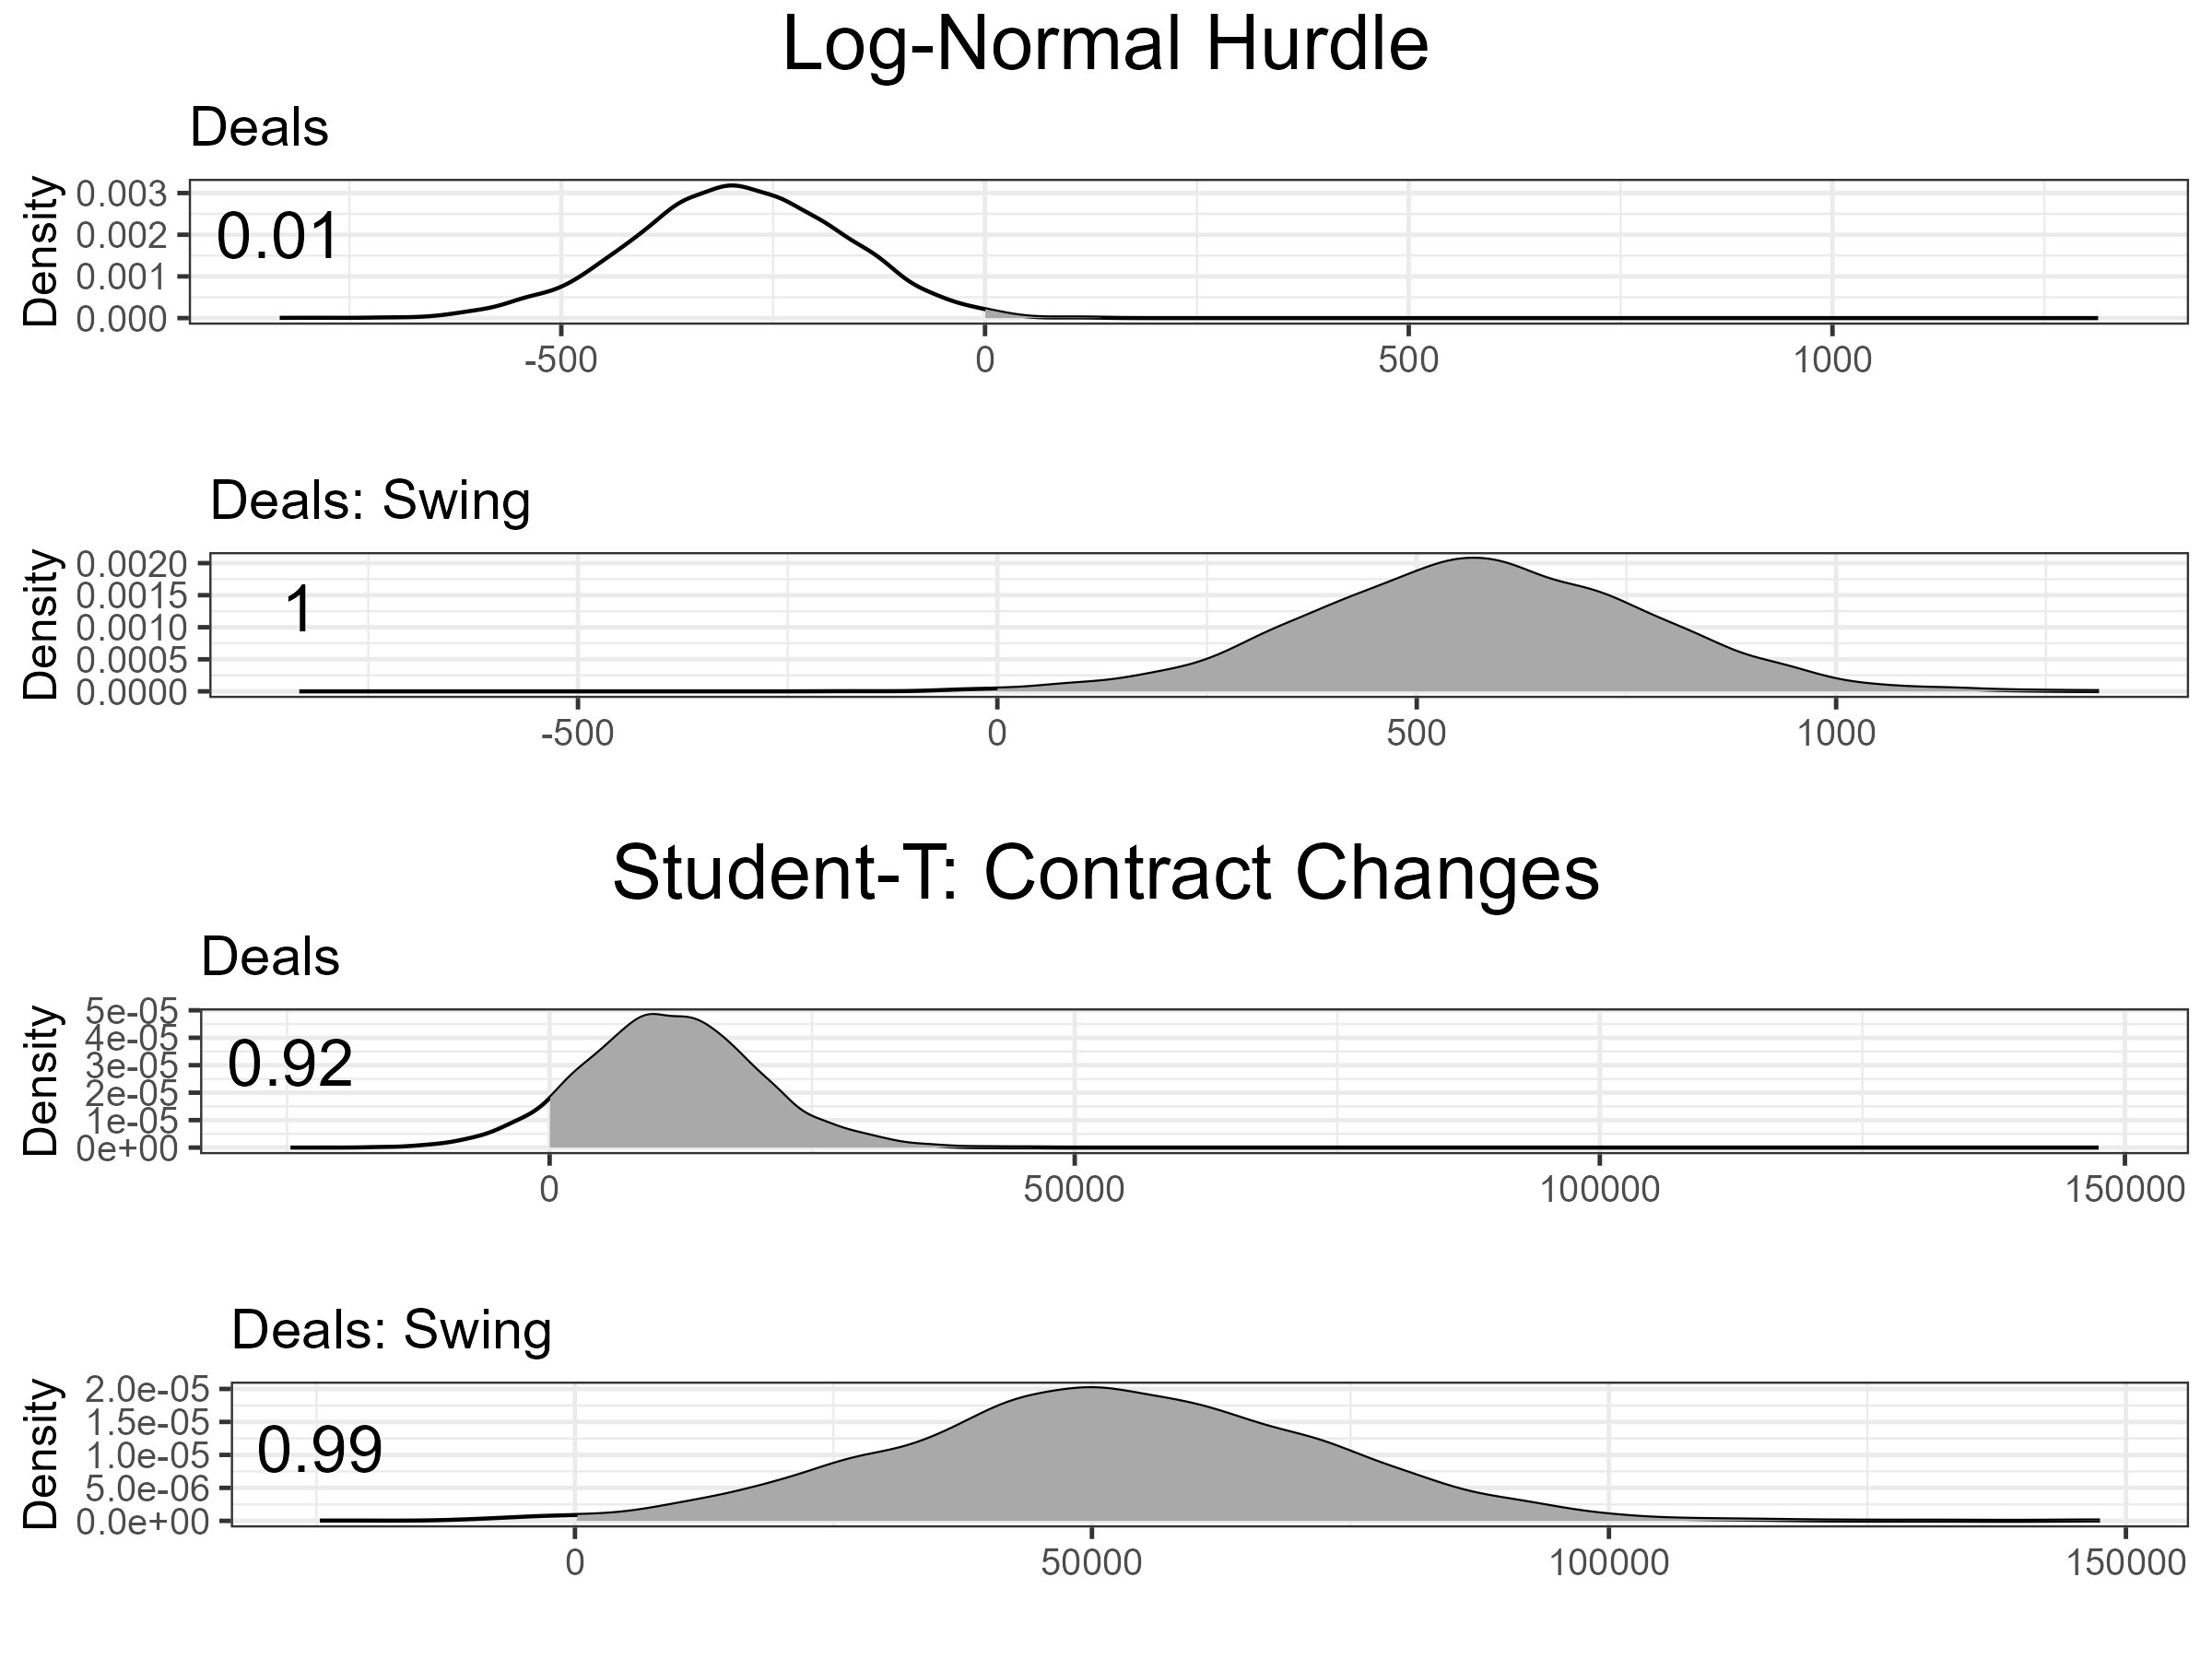
\includegraphics[width=0.95\textwidth]{me-deals-check.png}
	\caption{Shaded area and text give the positive posterior mass of each coefficient.}
	\label{fig:me-deals-check}
\end{figure}


A second approach uses the difference in contracts for each state in every year as the outcome. 
Because this measure is not normally distributed and has long tails, I use a student-t outcome distribution.
The student-t model also omits the state-specific lagged dependent variable, because using changes eliminates some of those dynamics. 


Results from the student-t model of contract changes also suggest that arms deals increase contract awards to swing states. 
99\% of the posterior mass in the interaction coefficient between deals and states is positive.
While 92\% of the posterior mass in the deals term is positive, which suggests increased deals lead to increased changes in contracts for other states as well, there is a 95\% posterior probability that the relationship between arms deals and contracts in swing states is larger. 
As a result, arms deals increase defense contracts more in swing states than in other states. 


\newpage 

\section{Additional Mechanism Check}

Here, I check the connection between deals and swing state contracts in another way. 
The arms deals models show that deals with autocracies increase as presidential elections approach. 
If those deals go to swing state contracts, then the marginal impact of deals on contracts in swing states should increase as presidential elections approach. 


To check this, I alter the model of contracts in the manuscripts by interacting the time to election indicator with swing state dummy and arms deals. 
I then present the marginal effect of deals on defense contracts in \autoref{fig:deals-me-prox}. 


\begin{figure}[htpb]
	\centering
		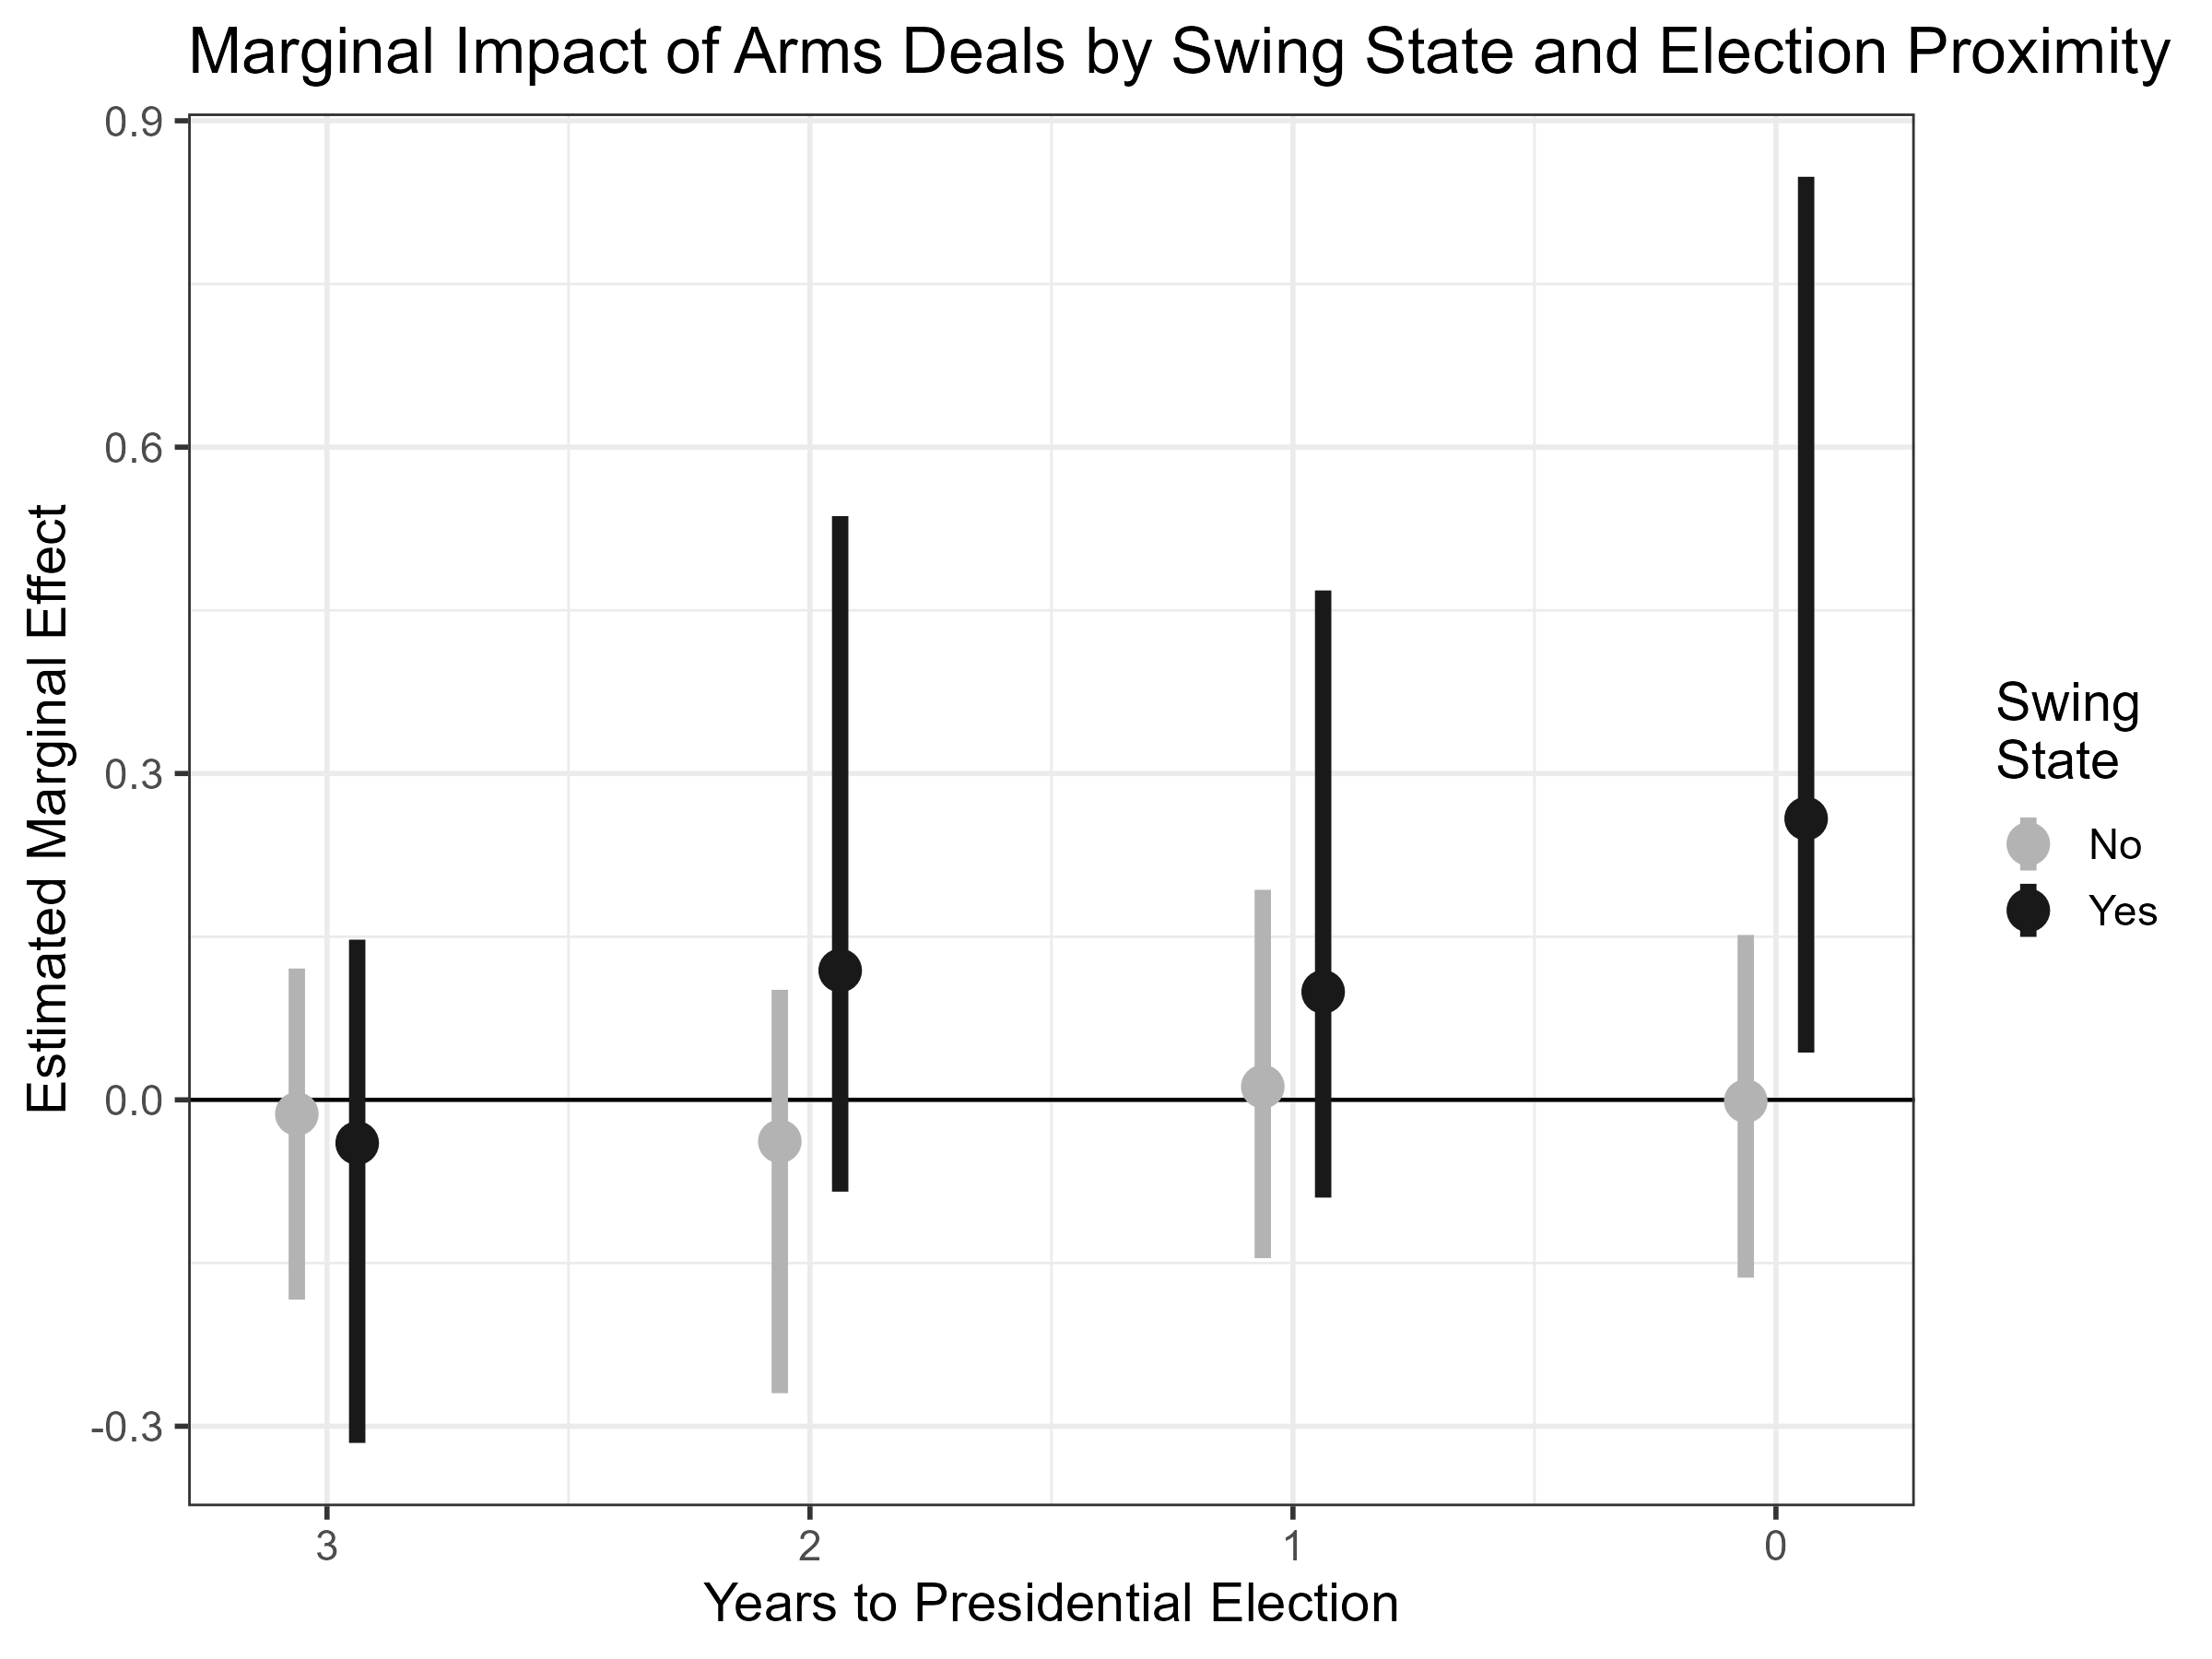
\includegraphics[width=0.95\textwidth]{deals-me-prox.png}
	\caption{Marginal effect of arms deals on defense contract awards based on swing state status and presidential election proximity. Estimates in millions of dollars.}
	\label{fig:deals-me-prox}
\end{figure}


The marginal impact of arms deals on contracts increases as presidential elections approach, but only in swing states. 
After an election, deals do not increase contracts in any state. 
But as elections approach, the marginal impact of deals on swing state contracts increases and is clearly positive in the year before and year of a presidential election. 
There is no clear impact of deals non-swing state contracts at any point in the electoral cycle. 
This implies that arms deals near elections feed increased swing state contracts. 


\newpage

\section{Coefficient Estimates}

The section presents tables with coefficient estimates. 
\autoref{tab:pois-regs} summarizes the hurdle Poisson coefficient estimates.\footnote{All tables built with modelsummary \citep{ArelBundock2022}}. 
\autoref{tab:cont-regs} summarizes the three deals models.


\begin{table}[H]

\caption{\label{tab:pois-regs}: Coefficient estimates from Poisson models of US arms deals.}
\centering
\resizebox{\linewidth}{!}{
\fontsize{8}{10}\selectfont
\begin{tabular}[t]{lcccc}
\toprule
  & Generic Cycle & Regime Cycle (No Controls) & Regime Cycle & Regime and Ally Cycle\\
\midrule
Hurdle: Intercept & 6 &  & 5 & 5\\
 & (4, 7) &  & (3, 6) & (3, 6)\\
Intercept & -1.0 & -0.13 & -0.8 & -0.66\\
 & (-1.5, -0.4) & (-0.19, -0.06) & (-1.4, -0.2) & (-1.28, -0.04)\\
Years to Election & -0.03 & -0.07 & -0.09 & -0.17\\
 & (-0.05, -0.01) & (-0.11, -0.03) & (-0.13, -0.06) & (-0.24, -0.09)\\
US Ally & 0.8 &  & 0.8 & 0.6\\
 & (0.7, 0.8) &  & (0.8, 0.9) & (0.4, 0.7)\\
Polyarchy & -0.07 & 0.9 & -0.2 & -0.6\\
 & (-0.15, 0.01) & (0.8, 1.0) & (-0.3, -0.1) & (-0.9, -0.3)\\
Cold War & 0.2 &  & 0.2 & 0.2\\
 & (0.1, 0.3) &  & (0.1, 0.3) & (0.1, 0.3)\\
Global War on Terror & -0.15 &  & -0.15 & -0.15\\
 & (-0.23, -0.07) &  & (-0.23, -0.07) & (-0.23, -0.07)\\
EU Member & 0.2 &  &  & \\
 & (0.1, 0.3) &  &  & \\
Republican President & -0.009 &  & -0.02 & -0.02\\
 & (-0.053, 0.037) &  & (-0.06, 0.03) & (-0.06, 0.03)\\
Log GDP & -0.04 &  & -0.030 & -3e-02\\
 & (-0.06, -0.01) &  & (-0.056, -0.003) & (-5e-02, -7e-04)\\
Ongoing MID & -0.23 &  & -0.3 & -0.3\\
 & (-0.42, -0.05) &  & (-0.5, -0.1) & (-0.5, -0.1)\\
Log Population & 0.2 &  & 0.2 & 0.2\\
 & (0.2, 0.2) &  & (0.1, 0.2) & (0.1, 0.2)\\
Log Distance & -0.07 &  & -0.12 & -0.11\\
 & (-0.10, -0.04) &  & (-0.15, -0.09) & (-0.14, -0.08)\\
Common Language & 0.03 &  & 4e-02 & 0.048\\
 & (-0.01, 0.08) &  & (5e-05, 9e-02) & (0.006, 0.091)\\
Hurdle: US Ally & -2 &  & -2 & -2\\
 & (-2, -2) &  & (-2, -2) & (-2, -2)\\
Hurdle: Polyarchy & 0.5 &  & 0.4 & 0.4\\
 & (0.3, 0.7) &  & (0.2, 0.6) & (0.2, 0.6)\\
Hurdle: Ongoing MID & 0.7 &  & 0.6 & 0.7\\
 & (0.3, 1.1) &  & (0.2, 1.1) & (0.3, 1.1)\\
Hurdle: Log GDP & -0.2 &  & -0.16 & -0.16\\
 & (-0.3, -0.1) &  & (-0.23, -0.08) & (-0.23, -0.08)\\
Years to Election:Polyarchy &  & 0.068 & 0.11 & 0.17\\
 &  & (0.009, 0.129) & (0.05, 0.17) & (-0.01, 0.35)\\
Log Petrol Revenue &  &  & 0.010 & 0.009\\
 &  &  & (0.007, 0.013) & (0.006, 0.012)\\
Years to Election:US Ally &  &  &  & 0.10\\
 &  &  &  & (0.01, 0.19)\\
US Ally:Polyarchy &  &  &  & 0.5\\
 &  &  &  & (0.1, 0.8)\\
Years to Election:US Ally:Polyarchy &  &  &  & -0.09\\
 &  &  &  & (-0.28, 0.10)\\
\bottomrule
\multicolumn{5}{l}{\rule{0pt}{1em}\textit{Note: }}\\
\multicolumn{5}{l}{\rule{0pt}{1em}90\% Credible Intervals in parentheses.}\\
\end{tabular}}
\end{table}



\begingroup\fontsize{8}{10}\selectfont

\begin{longtable}[t]{lccc}
\caption{\label{tab:cont-regs}: Coefficient estimates from models of defense contract awards.}\\
\toprule
  & Rescaled Ordered Beta & Log-Normal Hurdle & Student-T: Contract Changes\\
\midrule
Intercept & -5.1 & 6.3 & 0.31\\
 & (-5.6, -4.6) & (5.7, 6.8) & (-3.56, 4.15)\\
Arms Deals & -0.00026 & -0.00209 & 0.081\\
 & (-0.00155, 0.00103) & (-0.00389, -0.00041) & (-0.033, 0.205)\\
Swing State & -0.290 & -0.56 & 0.079\\
 & (-0.535, -0.034) & (-0.92, -0.21) & (-3.901, 4.106)\\
Core State & 0.0424 & 0.079 & 0.016\\
 & (-0.0041, 0.0906) & (0.012, 0.146) & (-3.667, 3.806)\\
Global War on Terror & 0.013 & 0.26 & 0.76\\
 & (-0.058, 0.082) & (0.18, 0.35) & (-3.14, 4.62)\\
Time to Election & 0.00092 & -0.045 & 0.05\\
 & (-0.01649, 0.01748) & (-0.068, -0.022) & (-3.52, 3.57)\\
Republican President & 0.029 & -0.0082 & 1.2\\
 & (-0.024, 0.079) & (-0.0762, 0.0582) & (-2.7, 5.1)\\
Population (Rescaled) & 0.098 & -0.011 & -0.35\\
 & (-0.011, 0.207) & (-0.127, 0.106) & (-4.18, 3.52)\\
Log GDP & -0.082 & 0.37 & -0.24\\
 & (-0.181, 0.019) & (0.25, 0.49) & (-4.15, 3.59)\\
Arms Deals:Swing State & 1.9e-03 & 0.0041 & 0.367\\
 & (6.1e-06, 3.9e-03) & (0.0013, 0.0068) & (0.083, 0.647)\\
$\phi$ & 629 &  & \\
 & (565, 698) &  & \\
Hurdle: Intercept &  & -2.9 & \\
 &  & (-3.2, -2.6) & \\
Hurdle: Log GDP &  & -0.659 & \\
 &  & (-1.228, -0.065) & \\
$\sigma$ &  & 0.38 & 135\\
 &  & (0.37, 0.40) & (121, 151)\\
\bottomrule
\multicolumn{4}{l}{\rule{0pt}{1em}\textit{Note: }}\\
\multicolumn{4}{l}{\rule{0pt}{1em}90\% Credible Intervals in parentheses.}\\
\end{longtable}
\endgroup{}




\newpage
\singlespace
 
\bibliography{../../MasterBibliography} 


\end{document}